\section{Appendix}
We include here all proofs for the statements of our paper.

%%%%%%%%%%%%%%%%%%%%%%%%%%%
% SECTION 2
% infinite lambda terms
%%%%%%%%%%%%%%%%%%%%%%%%%%%

%\begin{proposition}[Uniqueness of almost-left-finite type]
%\label{proposition-almost-left-finite-unique}
%If $t \in \LAMBDA$, $\Pi:\Gamma \vdash t:A$ and  $\Pi':\Gamma' \vdash t:A'$ are two almost-left-finite
%proofs then $A = A'$.
%\end{proposition}

%08:56 19/06/2024
\begin{proof}(Proof of Uniqueness of almost-left-finite type, Prop. \ref{proposition-almost-left-finite-unique})
By induction on the sum of the length of the leftmost branch in $\Pi$ and $\Pi'$. These lengths are finite
because $\Pi$ and $\Pi'$ are assumed to be almost-left-finite. Let $r$ be the last rule of $\Pi$ and $r'$ be the
last rule of $\Pi'$.
\begin{enumerate}
\item
Assume $r = \weak$. Then $\Pi$ is obtained from a proof $\Pi_1:\Gamma_1 \vdash t:A$. 
By induction hypothesis on $\Pi_1$ and $\Pi'$ we conclude that $A = A'$.

\item
Assume $r \not = \weak$ and $r' = \weak$. 
Then $\Pi'$ is obtained from a proof $\Pi'_1:\Gamma_1 \vdash t:A$. 
By induction hypothesis on $\Pi$ and $\Pi'_1$ we conclude that $A = A'$.

\item
Assume  $r \not = \weak$ and $r' \not = \weak$. Then both $r$ and $r'$ are the typing rule for
the outermost constructor of $t$ and for some
$h=0,1,2$ the proof $\Pi$ has premises $\Pi_1, \ldots, \Pi_h$
and the proof $\Pi'$ has premises $\Pi'_1, \ldots, \Pi'_h$ (for the same $h$). 
We distinguish one case for each constructor.

\begin{enumerate}
\item
Assume $t = x^T$. Then $r=r'=\var$-rule and $A = A' = T$.

\item
Assume $t =0^\N$. Then $r=r'=0$-rule and $A = A' = \N$.

\item
Assume $t =\Succ(u)$. Then $r=r'=\Succ$-rule  and $\Pi_1:\Gamma \vdash u: \N$
and $\Pi_2:\Gamma' \vdash u:\N$ and $A = A' = \N$.

\item
Assume $t = f(u)$. Then $r=r'=\ap$-rule and $\Pi_1:\Gamma \vdash f:U \rightarrow A$
and $\Pi_2:\Gamma' \vdash f:U' \rightarrow A'$. By induction hypothesis on $\Pi_1$ and
$\Pi'_1$ we deduce that $(U \rightarrow A) = (U' \rightarrow A')$, in particular that $A = A'$.

\item
Assume $t = \lambda x^T.b$. Then $r=r'=\lambda$-rule and 
$\Pi_1:\Gamma \vdash b:B$
and $\Pi_2:\Gamma' \vdash b:B'$. By induction hypothesis on $\Pi_1$ and
$\Pi'_1$ we deduce that $B=B'$, in particular that $A = T \rightarrow B = T \rightarrow B' = A'$.

\item
Assume $t = \cond(f,g)$. Then $r=r'=\cond$-rule and $\Pi_1:\Gamma \vdash f:A$
and $\Pi_2:\Gamma' \vdash f:A'$. By induction hypothesis on $\Pi_1$ and
$\Pi'_1$ we deduce that $A = A'$.

\end{enumerate}
\end{enumerate}
\end{proof}

%%%%%%%%%%%%%%%%%%%%%%%%%%%
% SECTION 3
% trace
%%%%%%%%%%%%%%%%%%%%%%%%%%%


\section{The trace of the infinite $\lambda$-terms}
%19:34 27/03/2024
We define a notion of trace for possibly infinite $\lambda$-terms, 
describing how an input of type $\N$ is used when computing the output.
The first step toward a trace is defining a notion of \emph{connection} between arguments
of type $\N$ in the proof that $t$ is well-typed. 
To this aim, we need the notions of \emph{list of argument
 types} and of \emph{index of atomic types} for a term.

We sketch the notion of connection through an example.
Assume 
\[
  {x_1}^{A_1}:A_1,{x_2}^{A_2}:A_2 \vdash t[x_1,x_2]:B_3 \rightarrow \N
\]
Then the list of argument types of $t$
is $A_1, A_2, B_3$. $A_1,A_2$ are arguments with names $x_1, x_2$, while $B_3$ is an unnamed
argument (it will be denoted by some bound variable in $t$). 
The index of an $\N$-argument of $t$ is any $j \in \{1,2,3\}$ such that $A_j=\N$
or $B_j=\N$ respectively: in this case all integers $1,2,3$ are indexes of some $\N$-argument,
in general we can have argument with type different from $\N$.

Remark that for an open term $ t[x_1,x_2]$ we list among the ``argument types'' also the
types $A_1, A_2$ of the free variables. We motivate this terminology:
in a sense, $t$ is an abbreviation of the closed term $t' = \lambda  
{x_1}^{A_1},{x_2}^{A_2}.t: (  A_1,A_2,B_3 \rightarrow \N )$, and the argument types of $t'$ are
$A_1, A_2, B_3$ and they include $A_1, A_2$. 

Below is the formal definition of argument types for a term.


\begin{definition}[List of argument types of a term]
Assume that $\vec{A} = A_1, \ldots, A_n$, $\vec{B}=B_{n+1}, \ldots, B_{n+m}$, 
$\Gamma = \{\vec{x}:\vec{A}\}$,
and $\Gamma \vdash t: \vec{B} \rightarrow \N$.

\begin{enumerate}
\item
The \emph{list of argument types} of $t$ is $\vec{C} = \vec{A},\vec{B}$. 

\item
$A_1, \ldots, A_n$ are the \emph{named arguments}, with names $x_1, \ldots, x_n$.

\item
$B_{n+1}, \ldots, B_{n+m}$ are the \emph{unnamed arguments}.

\item
An \emph{index of an $\N$-argument} 
of $t$ is any $j \in \{1, \ldots, n+m\}$ such that $C_j = \N$.

\end{enumerate}
\end{definition}

We now define the connection between $\N$-arguments of subterms of $t$
in a proof $\Pi: t:\Gamma \vdash A$ of  $\LAMBDA$. The connection describes
how an input  moves through the infinite unfolding of the term.
The definition of  atom connection for a syntax including the binder $\lambda$ 
is the main contribution of this paper. 
%Two $\N$-argument are in
%connection if and only if they receive the same global input: local input are ignored.
%In many cases two corresponding argument types have the same index, but if we insert or remove
%free variables or arguments the index may change.
Before providing the general definition, we discuss the notion of connection through examples. 
We draw in the same color two $\N$-argument which are in connection. 

\begin{Eg}\label{eg:0}\rm
An example of  atom connection for some instance of the $\weak$-rule.
\[
\infer[(\weak)]{
  {x_1} : \bfColor{red}{\N},{x_2} : \bfColor{blue}{\N}, x_3:\bfColor{oldgold}{\N}
  \prove t : \bfColor{orange}{\N} \rightarrow \N
}{
  {x_1} : \bfColor{red}{\N},{x_2} : \bfColor{blue}{\N} 
  \prove t : \bfColor{orange}{\N} \rightarrow \N
}
\]
\end{Eg}
Remark that the type $\N$ of the variable $x_3$, colored in \bfColor{oldgold}{old gold} and 
introduced by weakening, is in connection with no type in the rule $\weak$.

%20:13 15/04/2024
\begin{Eg}\label{eg:1}%\rm
An example of  atom connection for some instance of the $\apnotvar$-rule.
We assume that $a$ is \emph{not} a variable.
\[
\infer[(\apnotvar)]{
  x_1 : \bfColor{red}{\N},{x_2} : \bfColor{blue}{\N}
  \prove f(a) : \bfColor{orange}{\N} \rightarrow \N
}{
  x_1 : \bfColor{red}{\N},{x_2} : \bfColor{blue}{\N}
  \prove f : \bfColor{oldgold}{\N}, \bfColor{orange}{\N} \rightarrow \N
  &
  x_1 : \bfColor{red}{\N}, x_2: \bfColor{blue}{\N} \prove a : \N
}
\]
\end{Eg}
Remark that the first unnamed argument of $f$ (colored in \bfColor{oldgold}{old gold}) 
is in connection with no argument in the rule $\apnotvar$.
The reason is that in the term $f(a)$,
the first argument of $f$ receives a value from the value $a$ which is local to the term $f(a)$,
does not receive a value from outside the term.
However, the first argument of $f$ can be in connection with some argument higher in the typing proof. 
%13:21 15/04/2024

We postpone examples with the rule $\apvar$.

\begin{Eg}\label{eg:2}%\rm
An example of  atom connection for the rule $\cond$.
\[
\infer[(\cond)]{
  {x_1} : \bfColor{red}{\N},{x_2} : \bfColor{blue}{\N}
  \prove \cond(f,g) : \bfColor{oldgold}{\N} \rightarrow \N
}{
  x_1 : \bfColor{red}{\N},{x_2} : \bfColor{blue}{\N} \prove f : \N
  &
  x_1:\bfColor{red}{\N}, x_2:\bfColor{blue}{\N} \prove g:\bfColor{oldgold}{\N} \rightarrow \N
}
\]
\end{Eg}
Remark that the first unnamed argument of $\cond(f,g)$ (colored in \bfColor{oldgold}{old gold}) 
is in connection the type of the first unnamed one of $g$ in the second premise,
but it has no connection with the first premise. 


\subsection{A formal definition of connection}
The definition of connection requires to define an injection 
\[
\ins:\N,\N \rightarrow\N
\]
We set $\ins(p,x)=x+1$ if $x \ge p+1$, and $\ins(p,x)=x$ if $x\le p$.
The role of $\ins$ is inserting one fresh index $p+1$ for a new argument type higher in the proof
connected to no argument in the conclusion.

\begin{definition}[Connection in a proof of  $\LAMBDA$]
Assume $\vec{A} = A_1, \ldots, A_n$, $\vec{B}=B_1, \ldots, B_m$, $\Gamma = \vec{x}:\vec{A}$,
and $\Gamma \vdash t:\vec{B} \rightarrow \N$.

For each $\N$-argument $k$ in $t$, for $t'=t$ or $t'$  immediate subterm of $t$ 
each $\N$-argument $k'$ in $t'$ we define the relation: ``$k',t'$ the successor of $k,t$". We require:
\begin{enumerate}
\item
if $t$ is obtained by a rule $\weak$ from $t'=t$, described by a map $\phi:\Gamma \rightarrow \Delta$,  
then $k = \phi(k')$.
\item
if $t=f(a)$ is obtained by a rule $\apnotvar$ (i.e., $a$ is not a variable) and $t'=f$ 
then $k' = \ins(n,k)$. If $t'=a$ then $k'=k$ and $k' \le n$.
\item
if $t=f(x_i^{A_i})$ is obtained by a rule $\apvar$ and $t'=f$ 
then $k' = \ins(n,k)$or $k'=n+1$ and $k=i$.
\item
if $t=\cond(f,g)$ and $t'=f$ 
then $k' = \ins(n,k)$. If $t'=g$ then $k'=k$.
\end{enumerate}
We require $k = k'$ in all other cases, 
which are: $\Succ $, $\lambda$. 
\\
No connection is defined for the rules $\var$, $0$.
\end{definition}

Below we include some examples. 
We draw in the same color two $\N$-argument which are in connection. 
In the case of the rule $\apvar$, an argument can be connected to two arguments above it.


\begin{Eg}\label{eg:3}%\rm
Atom connection for $\apvar$.
We assume that $x$ is a variable.
\[
\infer[(\apvar)]{
  x_1 : \bfColor{red}{\N},{x_2} : \bfColor{blue}{\N}, x_3  : \bfColor{oldgold}{\N}
  \prove f(x_3) : \bfColor{orange}{\N} \rightarrow \N
}{
  x_1 : \bfColor{red}{\N},{x_2} : \bfColor{blue}{\N}, x_3  : \bfColor{oldgold}{\N}
  \prove f : \bfColor{oldgold}{\N}, \bfColor{orange}{\N} \rightarrow \N
}
\]
\end{Eg}

Remark that the last variable in the conclusion of the rule
is in connection with the first unnamed argument of $f$ (colored in \bfColor{oldgold}{old gold}) 
in the premise, and with the variable with the same name in the premise: there are
two connections.

\begin{Eg}\label{eg:4}%\rm
Atom connection for  $\lambda$-rule.
We assume that $x$ is  a variable.
\[
\infer[(\ap)]{
  x_1: \bfColor{red}{\N}, x_2: \bfColor{blue}{\N}
  \prove \lambda x.b : \bfColor{oldgold}{\N} \rightarrow \N
}{
  x_1: \bfColor{red}{\N}, x_2: \bfColor{blue}{\N}, x:\bfColor{oldgold}{\N} \prove b : \N
}
\]
\end{Eg}
Remark that the first unnamed argument of $\lambda x.b$ (colored in \bfColor{oldgold}{old gold}) 
in the conclusion is in connection with the last variable type in the premise of the rule.
\\

Summing up, when
we move up in a $\apvar$-rule, the type of last free variable corresponds to the type of the first
unnamend argument.
When  we move up in a $\lambda$-rule it is the other way round. 

The connection on $\N$-arguments in a proof $\Pi:\Gamma\vdash t:A$ defines a graph $\Graph(\Pi)$ 
whose nodes are all pairs $(k,u)$, with $u$ subterm of $t$ and $k$ index of some $\N$-argument of  $u$.
$\Graph(\Pi)$ is finite when $t$ is regular.
A trace represents the movement of an input information through the infinite unfolding of a tree.
Formally, we define a trace as a (finite or infinite) path in the graph $\Graph(\Pi)$.

\begin{definition}[Trace for well-typed terms in $\LAMBDA$]
Assume $\Pi$ is any typing proof of $t \in \WTyped$.
\begin{enumerate}
\item
A path of $\Pi$ is any finite or infinite branch $\pi =(i_0, \ldots, i_n, \ldots)$ of $\Pi$.

\item
Assume $\pi =(t_0, \ldots, t_n, \ldots)$ is a path of $\Pi$, finite or infinite. 
A finite or infinite \emph{trace} $\tau$ of $\pi$ in $\Pi$ is a list 
$\tau =( (k_m,t_m), \ldots, (k_n,t_n), \ldots)$ such that for all $i=m,\ldots, n,\ldots$:
\begin{enumerate}
\item
$k_i$ is an index of some $\N$-argument of $t_i$
\item
if $i+1$ is an index of $\tau$ then $(k_{i+1},t_{i+1})$ is connected with $(k_i, t_i)$ in $\Pi$.
\end{enumerate}

\end{enumerate}
\end{definition}

The starting point of a trace could be different from the starting point of the path to which the trace belongs.

%20:50 15/04/2024
%10:35 24/04/2024
%12:28 30/04/2024

%%%%%%%%%%%%%%%%%%%%%%%%%%%
% SECTION 4
% CT-lambda
%%%%%%%%%%%%%%%%%%%%%%%%%%%



\section{The circular system $\CTlambda$}
We introduce  a condition call \emph{global trace condition} for all proofs $\Pi$ that the term $t$ is well-typed,
then the subset $\GTC$ of the set $\WTyped$ of well-typed terms of $\LAMBDA$ 
satisfying the global trace condition. $\GTC$ is a set of total recursive functionals. We use $\GTC$
as a semantics for the set $\CTlambda$ of circular $\lambda$-terms we will define.

$\CTlambda$ will be the regular terms of $\CTlambda$. 
$\CTlambda$ is a decidable set.
For the terms of $\CTlambda$ we will prove
strong normalization, church-rosser for the \quotationMarks{safe} part of a term, 
and the fact that every closed normal term of type
$\N$ is a numeral. 
As a consequence, all terms $\CTlambda$ will be interpreted as total functionals. 
\\

From the $\N$-argument connection we now define the global trace condition and the set of 
terms of $\GTC$  and of $\CTlambda$.



\begin{definition}[Global trace condition and terms of $\CTlambda$]
\label{definition-global-trace-condition}
\mbox{}
 \linebreak 
Assume $\tau =( (k_m,t_m), \ldots, (k_n,t_n), \ldots)$ 
is a trace of a path $\pi = (t_1, \ldots, t_n, \ldots)$ of $t \in \WTyped$. 
Assume $i=m,\ldots, n$.
\begin{enumerate}
\item
$\tau$ is progressing in $i$ if $t_i=\cond(f,g)$ for some $f$, $g$,
and $k_i$ is the index of the first \emph{unnamed} argument the $\cond$-rule, 
otherwise $\tau$ is not progressing in $i$.

\item
$t$ satisfies the global trace condition if for some typing proof $\Pi$,
of $t$, for all infinite paths $\pi$ of $t$ in $\Pi$,
there is some infinitely progressing path $\tau$ in $\pi$ and $\Pi$.
$\GTC$ is the set of well-typed terms $t \in \LAMBDA$ satisfying the global trace condition.

\item
$\CTlambda = \GTC \cap \Reg$: the cyclic $\lambda$-terms of 
$\CTlambda$ are all well-typed terms which are regular trees (having finitely many subtrees), 
and which satisfy the global trace condition.

\end{enumerate}
\end{definition}

The notion of global trace condition is defined through a universal quantification on proof 
$\Pi:\Gamma \vdash t:A$, and proofs $\Pi$ are possibly infinite objects and they form 
a non-countable sets.
Therefore we would expect that the global trace condition is not decidable. 
Surprisingly, global trace is decidable in polynomial space in $t$. The reason is that is some proof satisfies
the global trace condition then all proofs do, and for regular terms there is a typing proof
which is a finite graph and for which the global trace condition is decidable.

We believe that the global trace condition is decidable quite fast
for realistic $\lambda$-terms. Another nice feature of the global trace condition is that for 
$t \in \GTC$ we require that there is some proof $\Pi:\Gamma \prove t:A$ whose
infinite paths all have some infinite progressing trace. This proof is almost-left-finite, because
all leftmost paths from a sub-proof have no progress point and therefore are finite. 
We conclude that $t \in \GTC$ implies that $t \in \WTyped$: we can assign a unique type to $t$
with a \quotationMarks{meaningful proof}, that is, an almost-left-finite finite proof.

We include now some examples of cyclic $\lambda$-terms. We recall that they have to satisfy
$\GTC$, therefore they are almost-left-finite, and by definition they are regular.

%18:05 03/06/2024

%\section{Examples of terms of $\CTlambda$}

\subsection{The sum map}

A first example of term of  $\CTlambda$. 
We provide an infinite regular term $\Sum$ computing the sum on $\N$.
In this example, the type superscript $\N$ of variables $x^\N$, $z^\N$ is omitted.

\begin{Eg}
\label{example-sum}
We set $\Sum = \lambda x.\cond(x,\lambda z.\Succ(\Sum(x)(z)))$.
$\Sum$ is a regular term because it has finitely many subterms: 
\begin{center}
  $\Sum$,
  \quad
  $\cond(x,\lambda z.\Succ(\Sum(x)(z)))$,
  \quad
  $x$,
  \quad
  $\lambda z.\Succ(\Sum(x)(z))$,
 \quad
  $\Succ(\Sum(x)(z))$,
  \quad
  $\Sum(x)(z)$,
  \quad
  $\Sum(x)$,
  \quad
   z
\end{center}
$\Sum$ is well-typed by the following derivation, in which we have a back edge from the 
$\bfColor{oldgold}{\dagger}$ above to the $\bfColor{oldgold}{\dagger}$ below.
\[
\infer[\lambda]{
  \vdash \Sum:\N, \bfColor{oldgold}{\N} \rightarrow \N 
   \quad (\bfColor{oldgold}{\dagger})
}{
  \infer[\cond]{
    x : \N \vdash 
    \cond(x,\lambda z.\Succ(\Sum(x)(z))): \bfColor{oldgold}{\N} \rightarrow \N
     \quad (\bfColor{oldgold}{ \spadesuit})
  }{
    \infer[\var]{
      x : \N \vdash x : \N
    }{}
    &
    \infer[\lambda]{
      x:\N \vdash \lambda z.\Succ(\Sum(x)(z)): \bfColor{oldgold}{\N} \rightarrow \N  
      %\quad (\bfColor{oldgold}{ \spadesuit})
    }{
      \infer[\Succ]{
        x:\N, z : \bfColor{oldgold}{\N} 
        \vdash \Succ(\Sum(x)(z)): \N  
        % \quad (\bfColor{oldgold}{ \spadesuit})
      }{
        \infer[\apvar]{
          x:\N, z : \bfColor{oldgold}{\N} 
          \vdash \Sum(x)(z): \N
        }{
          \infer[\apvar]{
            x:\N,  z : \bfColor{oldgold}{\N}
            \vdash \Sum(x): \bfColor{oldgold}{\N} \rightarrow \N
          }{
            \infer[\weak]{
              x:\N,  z : \bfColor{oldgold}{\N}
              \vdash \Sum: \N, \bfColor{oldgold}{\N} \rightarrow  \N
            }{
              \infer*{\vdash \Sum: \N, \bfColor{oldgold}{\N} \rightarrow \N 
                \quad (\bfColor{oldgold}{\dagger})}{}
            }
          }
        }
      }
    }
  }
}
\]
\end{Eg}

We colored in \bfColor{oldgold}{old gold} one sequence of atoms $\bfColor{oldgold}{\N}$:
this is one trace of the proof.
The colored trace is the unique infinite trace, it is cyclic and it is infinitely progressing.
We marked $\bfColor{oldgold}{ \spadesuit}$ the only progress point of the only infinite trace.
The progress point is repeated infinitely many times.


%
%\begin{tikzpicture}
%  %\draw [help lines] (-3,-1) grid (9,7);
%  \coordinate (a) at (0,0) node at (a) {A};
%  \coordinate (c) at (0,5) node at (c) {C};
%  \draw (0,0) -- (0:2cm);
%  \draw (0,0) -- (30:3cm);
%  \draw (0,5) -- +(0:2cm);
%\end{tikzpicture}


%10:43 16/04/2024

\subsection{The Iterator}

\begin{Eg}
We define a term $\Iter$ of  $\CTlambda$ computing the iteration of maps on $\N$.
The term $\Iter$ is a normal term of type $(\N \rightarrow \N), \N,\N \rightarrow \N$ such that
$\Iter(f,a,n)=f^n(a)$ for all numeral $n \in \Num$. 
We have to solve the equations:

\begin{enumerate}
\item
$\Iter(f,a,0) \sim a$ 
\item
$\Iter(f,a,\Succ (t)) \sim f(\Iter(f,a,t))$
\end{enumerate}

where $f$, $a$ abbreviate $f^{\N\rightarrow\N}$ and $a^\N$.
We solve them with $\Iter = \lambda f, a.\iter$
where 
$$
\iter = \cond (a, \lambda x.f(\iter(x))):\N \rightarrow \N
$$ 
is a term in the context $\Gamma = (f:\N \rightarrow \N, a:\N)$.
\end{Eg}

\begin{proposition}
$\Iter \in \Reg \cap \WTyped \cap \GTC = \CTlambda$.
\end{proposition}

\begin{proof}
The term $\Iter$ is well-typed and regular by definition. 
We check the global trace condition. 
\\
We follow the unique infinite trace $\tau$ of the last unnamed argument $\N$ of $\Iter$ 
in the unique infinite path $\pi$ of $\Iter$. 
The trace $\tau$ moves from  $\Iter = \lambda f. \lambda a.\iter$
 to the first unnamed argument of the sub-term $\lambda a.\iter$, 
then to $a:\N$ in the context of $\iter = \cond (a, \lambda x.f(\iter(x)))$.
Then the infinite path $\pi$ and moves in this order to:
 $\lambda x.f(\iter(x))$, $f(\iter(x))$, $ \iter(x)$, $\iter$
In the meanwhile, $\tau$ progresses from $\cond$ to the second argument $\lambda x.f(\iter(x))$
of $\cond$, then moves to $x$ in the context of $f(\iter(x))$,
then to $x$ in the context $\iter(x)$, and eventually to $x$ in the context of $\iter$.
%10:30 24/03/24
In this moment the infinite path $\pi$ loops from $\iter$ to $\iter$. At each loop the trace $\tau$ 
progresses once. We conclude that $\tau$ infinitely progresses.
\end{proof}

The proof above includes a type inference from the term $\iter$ to itself.
We draw the type inference in the picture below. 
We have a back edge from the 
$\bfColor{oldgold}{\dagger}$ on the top to the $\bfColor{oldgold}{\dagger}$ in the bottom,
and we marked $\bfColor{oldgold}{ \spadesuit}$ the only progress point, which is cyclically repeated
in $\tau$.
We abbreviate $\Gamma = (f:\N \rightarrow \N, a:\N)$.
\[
%\infer[\lambda]{ %opening: \infer[\lambda]
%  \vdash \Iter:(\N \rightarrow \N), \N, \bfColor{oldgold}{\N} \rightarrow \N
% }{
%  \infer[\lambda]{ %opening: \infer[\lambda]
%  f:\N \rightarrow \N
%  \vdash \lambda a.\iter:\N, \bfColor{oldgold}{\N} \rightarrow \N
%  }
{
    \infer[\cond]{ %opening: \infer[\cond]
      \Gamma 
      \vdash \iter: \bfColor{oldgold}{\N} \rightarrow \N 
        \quad (\bfColor{oldgold}{ \spadesuit}, \bfColor{oldgold}{\dagger})
     }{ 
         \infer[\var]{
       \Gamma 
      \vdash a:\N}{}
     &
        {\ \ \ \ \ \ }
        {\infer[\lambda] %opening: \infer[\lambda]
         {
         \Gamma
          \vdash \lambda x.f(\iter(x)):\bfColor{oldgold}{\N} \rightarrow \N
         }{
         \infer[\ap]{ %opening: \infer[\ap]
           \Gamma, x:\bfColor{oldgold}{\N}
          \vdash f(\iter(x)):\N
           }{
          \infer[\var]{
       \Gamma, x:\N 
      \vdash f:\N \rightarrow \N}{}
           {\ \ \ \ \ \ \ \ \ \ \ \ }
           {\infer[\apvar] %opening: \infer[\apvar]
            {\Gamma, x:\bfColor{oldgold}{\N}
        \vdash \iter(x): \N 
             }{
          \infer[\weak]{\Gamma, x:\N
                                 \vdash \iter: \bfColor{oldgold}{\N} \rightarrow \N}
                                {\infer*{\Gamma
                                 \vdash \iter: \bfColor{oldgold}{\N} \rightarrow \N
                                  \ \ \ (\bfColor{oldgold}{ \dagger})}{}
             }
           }
          }
        }%closing: \infer[\apvar]
      }%closing: \infer[\ap]
    }%closing: \infer[\lambda]
   }%closing: \infer[\cond]
 }%closing: \infer[\lambda]
%}%closing: \infer[\lambda]
\]




\subsection{The Interval Map}
A third example. We simulate lists with two variables $\nil:\alpha$ and 
$\cons:\N,\alpha \rightarrow \alpha$. We recursively define a notation for lists by $[]=\nil$,
$a @ l=\cons(a,l)$ and $[a,\vec{a}] = a @ [\vec{a}]$. We add no elimination rules for lists, though,
only the variables $\nil$ and $\cons$. Elimination rules are not required in our example.

\begin{Eg}
We will define a term $\Interval$ with one argument $f:\N \rightarrow \N$ and three argument
$a,x,y:\N$ (we skip all type superscripts), such that 
\[
\Interval(f,a,n,m) \  \sim \ [f^n(a), f^{n+1}(a), \ldots, f^{n+m}(a)] \  : \ \alpha
\]
for all numeral $n,m \in \Num$. 
We have to solve the recursive equations 
\begin{center}
  $\Interval(f,a,n,0) \sim [f^n(a)]$
  \quad
  and
  \quad
  $\Interval(f,a,n,\Succ (m))  \sim f^n(a) @ \Interval(f,a,\Succ(n),m)$.
\end{center}
Assume $\iter = \cond (a, \lambda x.f(\iter(x))):\N \rightarrow \N$ is the term
in the context $(f:\N\rightarrow\N, a:\N)$ defined 
in the previous sub-section: in particular, $\iter(n) \sim f^n(a)$ for all $n \in \Num$.
We solve the recursive equation for $\Interval$ with $\Interval = \lambda f,a.\interval$,
where 
\[
\interval:\N,\N \rightarrow \alpha
\]
is a term in the context $(f:\N\rightarrow\N, a:\N)$ defined by 
\[
\interval 
\ \ \ = \ \ \ 
\lambda x.\cond (\base,  \lambda y.\inductive),
\]
where the base case and the inductive case are
\[
\base 
\ \ \ =\ \ \  
[\iter(x)]
\ \ \ =\ \ \ 
\cons(\iter(x),\nil)
\]
\[
\inductive 
\ \ \ = \ \ \ 
\iter(x) @ \interval(\Succ(x))(y)
\ \ \ = \ \ \  
\cons(\ \iter(x), \ \interval(\Succ(x))(y) \ )
\]
\end{Eg}

\begin{proposition}
$\Interval \in \Reg \cap \WTyped \cap \GTC = \CTlambda$.
\end{proposition}

\begin{proof}
The term $\Interval$ is well-typed and regular by definition. We check the global trace condition.
Any infinite path $\pi$ either moves to $\iter$, for which we already checked the global trace condition,
or cyclically moves from $\interval$ to $\interval$.
We follow the unique infinite 
trace $\tau$ of the last unnamed argument $\N$ of $\Interval$ inside this infinite path.
The trace $\tau$ moves to the last unnamed argument $\N$ of  
$\interval:\N,\N \rightarrow \N$, then to the last unnamed argument of
$\cond (\ [\iter(x)],  \  \lambda y.\iter(x) @ (\lambda x.\interval)(\Succ(x))(y) \ )$.
In this step $\tau$ progresses, and moves to 
the first unnamed argument of $\lambda y.\iter(x) @ (\lambda x.\interval)(\Succ(x))(y) \ )$,
then to $y:\N$ in the context of $\iter(x) @ (\lambda x.\interval)(\Succ(x))(y) \ )$.
After one $\apvar$ rule, the trace $\tau$ reaches the unique unnamed argument of 
$(\lambda x.\interval)(\Succ(x))$, then the last unnamed argument $\tau$ of $\interval$. 
From $\interval$ the trace $\tau$ loops. Each time $\tau$ moves from $\interval$ to $\interval$
then $\tau$ progresses once. We conclude that $\tau$ infinitely progresses.
\end{proof}
%14:27 24/04/2024

The proof above includes a type inference from the term $\interval$ to itself.
We draw the type inference in the figure \ref{figure-term-interval}. 
In this figure, we include a back edge from the 
$\bfColor{oldgold}{\dagger}$ on the top to the $\bfColor{oldgold}{\dagger}$ in the bottom,
and we marked $\bfColor{oldgold}{ \spadesuit}$ the only progress point, which is cyclically repeated
in $\tau$.
We abbreviate 
$\Sigma = (\nil:\alpha, \cons:\N,\alpha \rightarrow \N)$
and
$\Gamma = \Sigma,(f:\N \rightarrow \N, a:\N)$.

%PROOF SNAPSHOT
\begin{figure}
\label{figure-term-interval}

%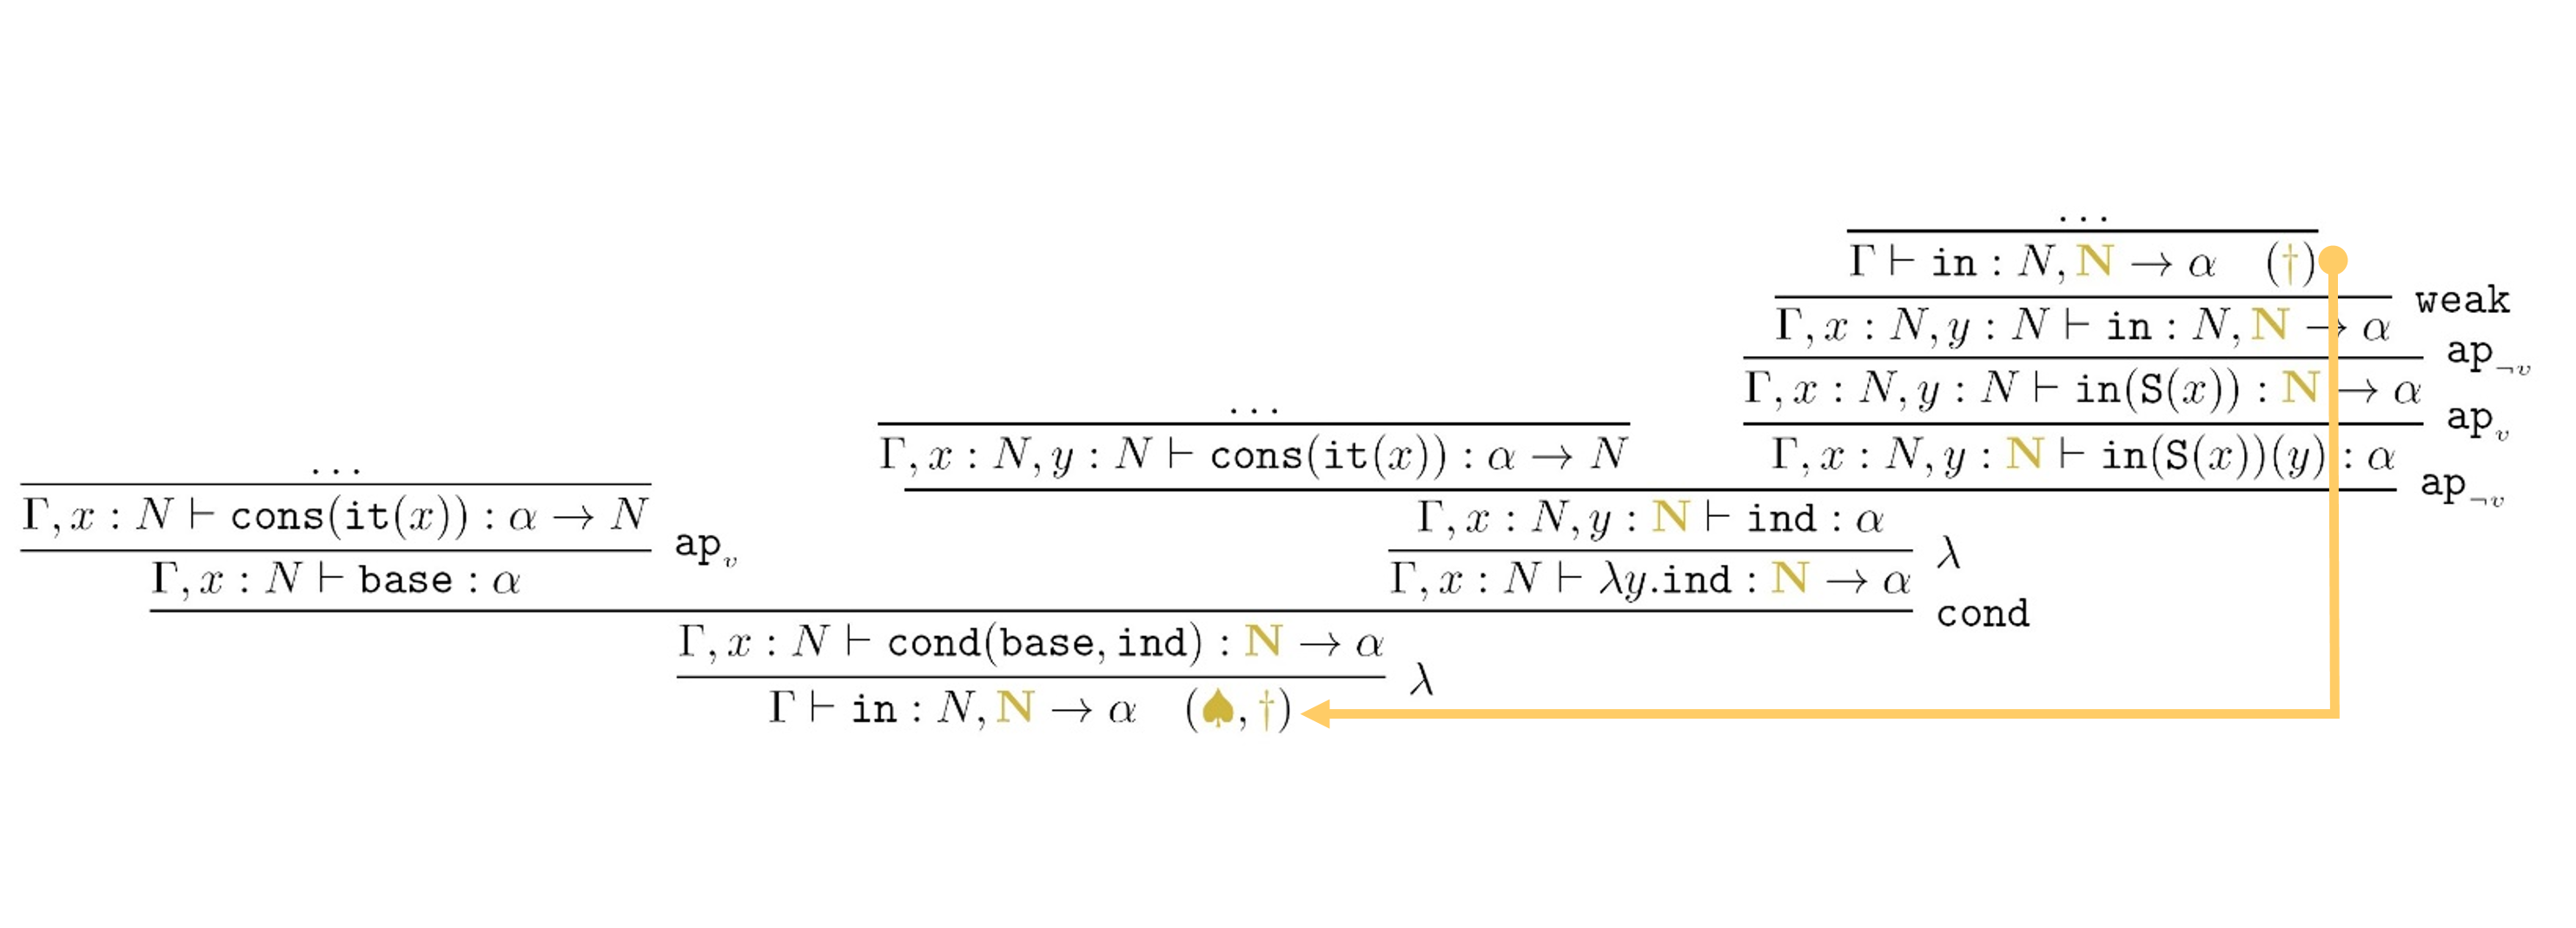
\includegraphics[scale=0.6]{type-inference-term-interval.PNG}

\begin{center}
%% LATEX SOURCE CODE THEN A SNAPSHOT 
%% THEN THE SNAPSHOT HAS BEEN MODIFIED IN WORD 
%% THEN A LAST SNAPSHOT
  
\[
%\infer[\lambda]
% {\Sigma\vdash \Interval:(\N \rightarrow \N),\N,\N,\bfColor{oldgold}{\N}\rightarrow\alpha}
% {\infer[\lambda]
%   {\Sigma,f:\N\rightarrow\N \vdash \lambda a.\interval:\N,\N,\bfColor{oldgold}{\N}   
%      \rightarrow\alpha}
   {\infer[\lambda]  
     {\Gamma \vdash \interval:\N,\bfColor{oldgold}{\N}\rightarrow\alpha 
       \ \ \ (\bfColor{oldgold}{\dagger}) }
       {\infer[\cond]{\Gamma, x:\N 
	\vdash 
	\cond (\base,  \inductive )
	:\bfColor{oldgold}{\N}\rightarrow\alpha \ \ \ (\bfColor{oldgold}{ \spadesuit}) } 
       {\infer[\apvar]{\Gamma, x:\N 
	           \vdash 
	           \base:\alpha}
             {\infer[]{\Gamma, x:\N 
	           \vdash 
	           \cons(\iter(x)):\alpha \rightarrow\N}{\ldots}}
            {\ \ \ \ \ \ }  &
          \infer[\lambda]{\Gamma, x:\N 
	           \vdash 
	           \lambda y.\inductive : \bfColor{oldgold}{\N}\rightarrow\alpha}
             {\infer[\apnotvar]{\Gamma, x:\N, y:\bfColor{oldgold}{\N} \vdash
               \inductive : \alpha}
            {\infer[]
                     {\Gamma, x:\N, y:\N 
                          \vdash \cons(\iter(x)):\alpha\rightarrow\N}{\ldots}
               {\ \ \ \ \ \ }
                     {\infer[\apvar]{\Gamma, x:\N, y:\bfColor{oldgold}{\N} 
                          \vdash \interval(\Succ(x))(y):\alpha}
                         {\infer[\apnotvar]{\Gamma, x:\N, y:\N 
                          \vdash \interval(\Succ(x)):\bfColor{oldgold}{\N} \rightarrow\alpha}
                              {\infer[\weak]{\Gamma, x:\N, y:\N 
                          \vdash \interval:\N,\bfColor{oldgold}{\N} \rightarrow\alpha}
                                {\infer[]{\Gamma 
                          \vdash \interval:\N,\bfColor{oldgold}{\N} \rightarrow\alpha
                           \ \ \ (\bfColor{oldgold}{\dagger})}
              {\ldots}}}}}
             }
           }
         }
       }  
    }
%   }
\]

\mbox{Figure \ref{figure-term-interval}}
\end{center}

\end{figure}

If we carefully examine the term $\Interval$, we can guess several results of this paper.
We have infinitely many nested $\beta$-reduction $(\lambda x. \ldots)(\Succ (x))$.
We can remove all of them in a single step. Inside the $\beta$-redex number $k$ we obtain a sub-term
$\iter[\Succ (x)/x]\ldots[\Succ (x)/x]$ (substitution repeated $k$ times).
The result is $\iter[\Succ ^k(x)/x] $.
The nested substitution produce infinitely many pairwise different sub-terms 
$\iter(\Succ ^k(x))$ for all $k \in \N$.
We need infinitely many steps to normalize all $\iter(\Succ ^k(x))$ to $f^k(I)$, 
even if we allow to reduce all $\beta,\cond$-redexes at the same time.
Also the normal form is not regular: it contains all terms $f^k(\iter(x))$ for $k \in \N$, hence
infinitely many pairwise different terms. 
%These infinite sub-terms are of a particulary simple form, though. 
%They are obtained by the repeating $k$ times the assignment $z:=f(z)$, then applying $z:=I$ once
%to the result.

In conclusion, 
$\Interval$ is some term of $\CTlambda$ which can be safely normalized, but which 
cannot be fully normalized in finite time, not even if we allow
infinite parallel reductions without any "safety" restriction. 
The normal form is produced \emph{only in the limit}
and it is \emph{not regular}. If we allow to reduce infinitely many nested existing
$\beta$-redexes in one step, also
the intermediate steps of the infinite reduction of $\Interval$ are not regular.


%16:32 30/04/2024
%22:30 03/06/2024


%%%%%%%%%%%%%%%%%%%%%%%%%%%
% SECTION 5
% subject reduction
%%%%%%%%%%%%%%%%%%%%%%%%%%%


\newcommand{\xx}{\boldsymbol{x}}

\section{Subject Reduction for Well-Typed Infinite Lambda Terms}
\label{section-subject-reduction}

We show the subject reduction for well-typed terms of $\LAMBDA$,
and also show the global trace condition is preserved by reductions. 
We first introduce some auxiliary notations for proofs of them.

Let $X$ be a set of variables of the form $x^T$.
We write $\Gamma_X$ for the sublist of $\Gamma$ consisting of all $x^T:T$ such that $x^T\in X$. 
Let $\Gamma$ and $\Delta$ be contexts of $\LAMBDA$.
The merged context $\mergeCtx{\Gamma}{\Delta}$
is defined by $\Gamma\conc(\Delta_{\FV(\Delta)\setminus\FV(\Gamma)})$. 

Let $\theta$ be a renaming, and 
$S_1 = \Gamma_1\vdash t_1:\vec{B_1}\rightarrow N$
and $S_2 = \Gamma_2[\theta]\vdash t_2[\theta]:\vec{B_2}\rightarrow N$ be sequents. 
Let $k_1$ and $k_2$ be indexes of $N$-arguments of $t_1$ and $t_2$, respectively. 
Then we write $(k_1,S_1) \simIndex{\theta} (k_2,S_2)$ (or $(k_1,t_1) \simIndex{\theta} (k_2,t_2)$ for short)
if they are respectively indexes of named arguments for some $y$ and $\theta(y)$, or
are respectively those of unnamed arguments at the same position $i$ in $\vec{B_1}$ and $\vec{B_2}$,
namely $k_1=|\Gamma_1|+i$ and $k_2=|\Gamma_2|+i$,
where $|\Gamma_1|$ and $|\Gamma_2|$ are the sizes of $\Gamma_1$ and $\Gamma_2$. 
Note that the index equivalent to $k_1$ is unique (if it exists), namely 
$(k_1,t_1) \simIndex{\theta} (k_2,t_2)$ and $(k_1,t_1) \simIndex{\theta} (k'_2,t_2)$ implies $k_2=k'_2$.
We write $(k_1,t_1) \simIndex{} (k_2,t_2)$ if $\theta$ is the identity renaming. 

In this paper we do not implicitly identify $\alpha$-equivalent terms,
in order to make simpler to state the global trace condition.
For this reason, proofs of this section requires some delicate treatment of variables.

We consider the following restricted $\lambda$ rule (called $\lambda'$) as follows:
\begin{itemize}
\item
  $\lambda'$-rule.
  If $\Gamma, x^A:A \vdash b: B$ and $\FV(\Gamma) = \FV(\lambda x.b)$, 
  then $ \Gamma \vdash \lambda x^A.b :A \rightarrow B$.
\end{itemize}

The next lemma says that if $\Gamma\vdash t:A$ is provable,
then $t:A$ can be shown in a restricted context $\Gamma_{\FV(t)}$
even if the rule $\lambda$ is restricted to $\lambda'$. 

\begin{lemma}\label{lem:thinning}
  Assume $\Pi:\Gamma\vdash t:A$.
  Then $\Pi':\Gamma_{\FV(t)}\vdash t:A$ for some $\Pi'$ that may have instances of the rule $\lambda'$
  and not have those of the rule $\lambda$.
  Moreover if the global trace condition holds for $\Pi$, then it also holds for $\Pi'$. 
\end{lemma}
\begin{proof}
  First we call the following admissible rule $\lambda'\weak$:
  \begin{itemize}
  \item
    $\lambda'\weak$-rule.
    If $\Gamma, x^A:A \vdash b: B$, $\FV(\Gamma) = \FV(\lambda x.b)$ and $\Gamma\subseteqsim \Gamma'$, 
    then $ \Gamma' \vdash \lambda x^A.b :A \rightarrow B$.
  \end{itemize}
  We write $\Rule'$ as the set of rule instances obtained by removing
  those of $\lambda$ from $\Rule$ and adding those of $\lambda'\weak$. 
  Note that if we have a proof of a sequent with $\lambda'\weak$,
  then we also have a proof of the same sequent not with $\lambda'\weak$
  by a proof transformation that splits each $\lambda'\weak$ by $\lambda'$ and $\weak$. 
  Also note that this proof transformation preserves the global trace condition.

  Let $\Pi$ be $(T,\phi)$.
  For each $l \in T$, we write $\Gamma_l\vdash t_l:A_l$
  for the conclusion of $\phi(l) \in \Rule$. 
  To show the lemma, from a given proof $\Pi$, 
  it is enough to construct a proof $\Pi'$ of $\Restrict{\Gamma}{\FV(t)}\vdash t:A$ with $\Rule'$.
  
  We define the set of nodes of $\Pi'$ is $T$, which is the same one of $\Pi$. 
  For each $l\in T$, we define $\phi'(l)$ and $\Gamma'_l$ that satisfies
  the following requirements:
  \begin{itemize}
  \item[(a)]
    $\Gamma'_l\vdash t_l:A_l$ is the conclusion of $\phi'(l) \in \Rule'$,
  \item[(b)]
    $\Restrict{(\Gamma_l)}{\FV(t_l)} \subseteqsim \Gamma'_l \subseteqsim \Gamma_l$
    and $\Gamma'_{\nil} = \Restrict{\Gamma}{\FV(t)}$, 
  \item[(c)]
    if $\tilde{k},t_{l\conc(i)}$ is the successor of $k,t_l$ in $\Pi$
    and $k$ is an index of some unname argument
    or a named argument of some name $z\in\FV(t_l)$, 
    then there are $\tilde{k'}$ and $k'$ such that
    $\tilde{k'},t_{l\conc(i)}$ is the successor of $k',t_l$ in $\Pi'$, 
    $(k,t_l) \simIndex{} (k',t_l)$,
    and $(\tilde{k},t_{l\conc(i)}) \simIndex{} (\tilde{k'},t_{l\conc(i)})$.
    Moreover, if $k$ is an index of a progressing argument, then so is $k'$.
  \end{itemize}
  Note that the proof is done if we construct $\Pi'$ that satisfies these requirements. 
  
  We define $\Gamma'_{\nil} = \Restrict{\Gamma}{\FV(t)}$.
  Then it satisfies (b) since $t_\nil = t$. 
  Next, assuming the induction hypothesis that $\Gamma'_l$ which satisfies (b)
  is already defined, 
  we define $\phi'(l)$ and $\Gamma_{l\conc(i)}$, 
  for each $i$ such that $l\conc(i)\in T$, 
  that satisfies (a), (b), and (c). 
  It is done by the case analysis of $\phi(l)$.

  The case of $\phi(l) = \Gamma_l\vdash x:A_l$,
  which is an instance of the rule $\var$ with $x:A_l\in\Gamma_l$. 
  Then define $\phi'(l) = \Gamma'_l\vdash x:A_l$. This is an instance of $\var$
  because $x:A_l \in \Restrict{(\Gamma_l)}{\FV(x)} \subseteqsim \Gamma'_l$ by (b).

  The case of $\phi(l) = (\Gamma_{l\conc(1)}\vdash t_l:A_l,\Gamma_{l}\vdash t_l:A_l)$,
  which is an instance of the rule $\weak$ with
  $t_{l\conc(1)} = t_l$, $A_{l\conc(1)} = A_{l}$, and
  $\Gamma_{l\conc(1)}\subseteqsim \Gamma_l$.
  Let $\psi$ be the unique map that determines $\Gamma_{l\conc(1)}\subseteqsim \Gamma_l$.
  Then define $\Gamma'_{l\conc(1)}$ such that
  $\Gamma'_{l\conc(1)}\subseteqsim \Gamma'_l$ determined by
  the induced map from $\psi$ restricting the range to $\FV(\Gamma'_l)$.
  Note that $\FV(\Gamma'_{l\conc(1)}) = \FV(\Gamma'_l)\cap\FV(\Gamma_{l\conc(1)})$. 
  Then it satisfies (b) since $\FV(t_l)\subseteq \FV(\Gamma'_l) \cap \FV(\Gamma_{l\conc(1)}) = \FV(\Gamma'_{l\conc(1)}) \subseteq \FV(\Gamma_{l\conc(1)})$ by (b) for $\Gamma'_l$.
  Define $\phi'(l) = (\Gamma'_{l\conc(1)}\vdash t_l:A_l,\Gamma'_{l}\vdash t_l:A_l)$
  as an instance of the rule $\weak$. 
  Hence the requirement (a) holds.
  We can also show (c): if $k$ is an index in $\Gamma_l\vdash t_l:A_l$ for a name
  $z\in\FV(t_{l\conc(1)}) = \FV(t_l)$, then we can take an index $k'$
  in $\Gamma'_l\vdash t_l:A_l$ for $z$ by $\FV(t_l)\subseteq\FV(\Gamma'_l)$ by (b). 
  An index $\tilde{k'}$ for the name $z$ can be taken
  from $\Gamma'_{l\conc(1)}\vdash t_l:A_l$
  since $z \in \FV(t_l) \subseteq \FV(\Gamma'_{l\conc(1)})$. 
  
  The case of $\phi(l) = (\Gamma_l,z:C\vdash b:\vec{B}\to N, \Gamma_l\vdash\lambda z^C.b:C,\vec{B}\to N)$
  that is an instance of the rule $\lambda$. 
  Define $\Gamma'_{l\conc(1)} = \Restrict{(\Gamma_l)}{\FV(\lambda z.b)},z:C$ and 
  $\phi'(l) = (\Restrict{(\Gamma_l)}{\FV(\lambda z.b)},z:C\vdash b:\vec{B}\to N, \Gamma'_l\vdash \lambda z.b:C,\vec{B}\to N)$. 
  This is an instance of the rule $\lambda'\weak$, since $\Restrict{(\Gamma_l)}{\FV(\lambda z.b)}\subseteqsim \Gamma'_l$ by the induction hypothesis.
  Trivially we have (a). 
  We also have (b) by $\Restrict{(\Gamma_l,z:C)}{\FV(b)} \subseteqsim (\Restrict{(\Gamma_l)}{\FV(\lambda z.b)},z:C) \subseteqsim (\Gamma_l,z:C)$.   
  The requirement (c) holds: 
  if $k$ is an index of some named argument $y\in\FV(\lambda z.b)$ in $\Gamma_l$,
  then $k'$ can be taken as the index of $y$ in $\Gamma'_l$ by (b) for $\Gamma_l$.
  If $k$ is an index of some unnamed argument in $C,\vec{B}$,
  then $k'$ can be taken as the index of some unnamed argument. 
  In both cases, their successors $\tilde{k}$ and $\tilde{k'}$ are uniquely
  determined by $k$ and $k'$, respectively. 
  
  The case that $\phi(l)$ is an instance of the rule $\apvar$
  whose conclusion is $\Gamma_l\vdash f(x^B):\vec{C}\to N$ with $x:B\in \Gamma_l$.  
  Define $\Gamma'_{l\conc(1)} = \Gamma'_l$.
  This satisfies (b) by the induction hypothesis. 
  Then define
  $\phi'(l) = (\Gamma'_{l\conc(1)}\vdash f:B,\vec{C}\to N, \Gamma'_l\vdash f(x^B):\vec{C}\to N)$
  as an instance of the rule $\apvar$. This satisfies (a). 
  In order to show (c), 
  take an index $k$ for $\Gamma_l\vdash f(x^B):\vec{C}\to N$, which is the one for
  a named argument $y \in \FV(f(x^B))$ in $\Gamma_l$
  or for some unnamed argument of $\vec{C}$. 
  For the latter case, the indexes $\tilde{k}$, $k'$ and $\tilde{k'}$ can be taken
  as those of the unnamed argument in $\vec{C}$ at the same position as $k$.
  For the former case, we take $k'$ as the index for $y$ in $\Gamma'_l$.
  In order to take $\tilde{k'}$,
  we further have two subcases according to $\tilde{k}$: 
  The first one is $\tilde{k}$ is the index for the same named argument as $k$, 
  and the second one is $\tilde{k}$ is the index for the unnamed argument, namely $B=N$.
  In both subcases, we can take the equivalent $\tilde{k'}$ to $\tilde{k}$ as we wished.
    
  The case that $\phi(l)$ is an instance of the rule $\apnotvar$
  whose conclusion is $\Gamma_l\vdash f(b^B):A_l$. 
  Define $\Gamma'_{l\conc(1)} = \Gamma'_{l\conc(2)} = \Gamma'_l$.
  This satisfies (b) by the induction hypothesis.
  Then define $\phi'(l) = (S_1, S_2, \Gamma'_l\vdash f(b^B):\vec{C}\to N)$,
  where $S_1$ is $\Gamma'_{l}\vdash f:B,\vec{C}\to N$
  and $S_2$ is $\Gamma'_{l}\vdash b:B$, as an instance of $\apnotvar$.
  This satisfies (a).
  In order to show (c), 
  take an index $k$ for $\Gamma_l\vdash f(x^B):\vec{C}\to N$, which is the one for
  a named argument $y \in \FV(f(x^B))$ in $\Gamma_l$
  or for some unnamed argument of $\vec{C}$.
  For the former case, the successor $\tilde{k}$ of $k$ is uniquely taken.
  By $\FV(f(b)) \subseteq \FV(\Gamma'_l)$, the index $k'$ equivalent to $k$ is uniquely taken. 
  Then the successor $\tilde{k'}$ of $k'$ is also taken as we wished. 
  For the latter case, the successor $\tilde{k}$ of $k$ is uniquely taken
  as the one for unnamed argument at the same position as $k$. 
  Then $k'$ equivalent to $k$ is uniquely taken, and 
  its successor $\tilde{k'}$ is also taken as we wished. 

  The case that $\phi(l)$ is an instance of the rule $0$
  whose conclusion is $\Gamma_l\vdash 0:N$. 
  Define $\phi'(l) = \Gamma'_l\vdash 0:N$ as an instance of the rule $0$.
  This satisfies the requirements (a), (b), and (c). 

  The case that $\phi(l)$ is an instance of the rule $\Succ$
  whose conclusion is $\Gamma_l\vdash \Succ(t_{l\conc(1)}):N$ with $A_l=N$.
  Define $\Gamma'_{l\conc(1)} = \Gamma'_l$, and 
  $\phi'(l) = (\Gamma'_l\vdash t_{l\conc(1)}:N, \Gamma'_l\vdash \Succ(t_{l\conc(1)}):N)$
  as an instance of $\Succ$. They satisfy (a) and (b). 
  The requirement (c) is also satisfied:
  Take an index $k$ for $\Gamma_l\vdash \Succ(t_{l\conc(1)}): N$,
  which is the one for a named argument $y \in \FV(\Succ(t_{l\conc(1)})$ in $\Gamma_l$.
  Then the successor $\tilde{k}$ of $k$ is uniquely taken.  
  By $\FV(t_{l\conc(1)}) \subseteq \FV(\Gamma'_l)$, the index $k'$ equivalent to $k$ is uniquely taken. 
  Then the successor $\tilde{k'}$ of $k'$ is also taken as we wished. 
  
  The case that $\phi(l)$ is an instance of the rule $\cond$
  whose conclusion is $\Gamma_l\vdash \cond(f,g):N,\vec{C}\to N$. 
  Define $\Gamma'_{l\conc(1)} = \Gamma'_{l\conc(2)} = \Gamma'_l$, and 
  $\phi'(l) = (S_1,S_2, \Gamma'_l\vdash \cond(f,g):N,\vec{C}\to N)$,
  where $S_1$ is $\Gamma'_l\vdash f:\vec{C}\to N$ and $S_2$ is $\Gamma'_l \vdash g:N,\vec{C}\to N$, 
  as an instance of $\cond$. They satisfy (a) and (b). 
  To show (c), take an index $k$ for $\Gamma_l\vdash \cond(f,g): N,\vec{C}\to N$ as required. 
  We need to consider three cases:
  $k$ is the index for a named argument $y \in \FV(\cond(f,g))$ in $\Gamma_l$,
  is the one for an unnamed argument in $\vec{C}$, or
  is the one for an unnamed argument in $N$ (the first one of $N,\vec{C}\to N$). 
  For the first and second cases, we can take $\tilde{k}$, $k'$, and $\tilde{k'}$
  similar to the other cases.
  For the last case, the successor $\tilde{k}$ of $k$ should be taken
  as the index of the unnamed $N$-argument of $\Gamma'_l \vdash g:N,\vec{C}\to N$
  at the same position as $k$. 
  Then $k'$ and $\tilde{k'}$ are taken as those equivalent to $k$ and $\tilde{k}$, respectively.
  Note that this $k$ is an index of a progressing argument $N$, and so is $k'$. 
\end{proof}



\begin{lemma}[Substitution lemma]
  Assume that $\Pi_u: \Delta \vdash u:A$ and $\Pi_t:\Gamma,x:A \vdash t:B$ hold. 
  Then there exists $\Pi^\circ$ such that $\Pi^\circ:\mergeCtx{\Delta}{\Gamma} \vdash t[u/x]:B$. 
  Moreover, if both $\Pi_u$ and $\Pi_t$ satisfy the global trace condition,
  then $\Pi^\circ$ also satisfies it. 
\end{lemma}
\begin{proof}
  Assume that $\Pi_u: \Delta \vdash u:A$ and $\Pi_t:\Gamma,x:A \vdash t:B$ hold. 
  By Lemma~\ref{lem:thinning}, without loss of generality,
  we can assume $\FV(\Delta) = \FV(u)$ and $\Pi_t$ is a proof with the restricted $\lambda$ rule (the $\lambda'$ rule). 
  Let $\Pi_u=(T_u,\phi_u)$ and $\Pi_t=(T_t,\phi_t)$.
  For each $l\in T_t$, we write $\Gamma_l\vdash t_l:C_l$
  for the conclusion of $\phi_t(l)$.
  We use $\xx$ to mark occurences of $x$ in $\Pi_t$ that connects
  with the explicit $\xx$ of $\Gamma,\xx:A\vdash t:B$. 
  In the following, we construct a proof $\Pi^\circ = (T^\circ,\phi^\circ)$ of
  $\mergeCtx{\Delta}{\Gamma}\vdash t[u/x]:B$ such that 
  \begin{itemize}
  \item[(a1)]
    $T^\circ = T_t \cup T_{\var} \cup T_{\apvar}$, where
    $T_{\var} = \{l\conc(1)\conc l' \mid \text{$l\in T_t$, $\phi(l)=\var$ of $\xx$, and $l'\in T_u$} \}$
    and
    $T_{\apvar} = \{l\conc(2)\conc l' \mid \text{$u$ is not a variable, $l\in T_t$, $\phi(l)=\apvar$ of $f(\xx)$ for some $f$, and $l'\in T_u$}\}$.
    The explicit $1$ of $l\conc(1)\conc l' \in T_\var$ is called the switching point of $l\conc(1)\conc l'$.
    The explicit $2$ of $l\conc(2)\conc l' \in T_\apvar$ is also called the switching point of $l\conc(2)\conc l'$.     \item[(a2)]
    For each $l\conc(i)\conc l' \in T_\var \cup T_\apvar$ with switching point $i$,
    we have $\phi^\circ(l\conc(i)\conc l') = \phi_u(l')$. 
  \end{itemize}
  Moreover, for all $l \in T_t$,
  the rule instance $\phi^\circ(l)$ satisfies the following requirements
  with an auxiliary function $\sigma^\circ:T_t \to \Seq$ and a substitution $\theta_l$: 
  \begin{itemize}
  \item[(b1)]
    The sequent $\sigma^\circ(l)$ has the form $\Gamma^\circ_l\vdash t_l[\theta_l]:C_l$.
    The substitution $\theta_l$ is $\{u/\xx\}\cup\theta_{{\rm ren}}$
    if $\xx:A \in \Gamma_l$, and is $\theta_{{\rm ren}}$ otherwise, 
    where $\theta_{{\rm ren}}$ is some renaming.
    $\Gamma^\circ_l \sim \Delta_l\sharp\Restrict{(\Gamma_l)}{\overline{\xx}}[\theta_l]$ holds,
    where $\Delta_l$ is $\Delta$ if $\xx:A\in\Gamma_l$, and is $\emptyset$ otherwise. 
  \item[(b2)]
    $\sigma^\circ(l)$ is the conclusion of $\phi^\circ(l)$,
    and $\sigma^\circ(l\conc(i))$ is the $i$-th assumption of $\phi^\circ(l)$ if $l\conc(i) \in T_t$.
  \item[(b3)]
    Assume $\tilde{k},t_{l\conc(i)}$ is a successor of $k,t_l$ and $k$ is not a named index for $\xx$. 
    Then there exist $\tilde{k^\circ}$ and $k^\circ$ such that
    $\tilde{k^\circ},t_{l\conc(i)}[\theta_{l\conc(i)}]$ is a successor of $k^\circ,t_l[\theta_l]$ and 
    $(k,t_l) \simIndex{\Restrict{(\theta_l)}{\overline{\xx}}} (k^\circ,t_l[\theta_l])$.
    If $k$ is an index of a progressing argument, then so is $k^\circ$.    
  \end{itemize}
  
  Note that if we have $\Pi^\circ$ that satisfies the requirements, its possibly infinite path
  is a path of $\Pi_t$ or a path of $\Pi_u$ or a path $l\conc(i)\conc l'$,
  where $l$ is a path of $T_t$, $i$ is a switching point, and $l'$ is a path of $T_u$.
  Hence $\Pi^\circ$ is Almost-left-finite, since $\Pi_t$ and $\Pi_u$ are Almost-left-finite.
  In addition, if $\Pi_t$ and $\Pi_u$ satisfies the global trace condition,
  so is $\Pi^\circ$ by (b3). 
  Therefore, to complete the proof, it is enough to construct $\Pi^\circ$. 

  First, for each $l\conc(j)\conc l'\in T_\var\cup T_\apvar$ with a switching point $j$, 
  we define $\phi^\circ(l\conc(j)\conc l') = \phi_u(l')$. 

  In the following, for each $l\in T_t$, we inductively define $\Gamma^\circ_l$, $\phi^\circ(l)$, and $\sigma(l)$
  that satisty (b1), (b2), and (b3).
  The case of $l=\nil$, define $\Gamma^\circ_\nil = \Delta\sharp\Gamma$ and $\theta_\nil=\{u/\xx\}$,
  and define $\sigma^\circ(\nil)$ as $\mergeCtx{\Delta}{\Gamma}\vdash t[u/\xx]:A$. 
  Hence we have (b1) since
  $\Gamma^\circ_\nil = \mergeCtx{\Delta}{\Gamma} \sim \mergeCtx{\Delta}{\Restrict{(\Gamma,\xx:A)}{\overline{\xx}}[\theta_\nil]}$. 

  For each $l\in T_t$,
  with the induction hypothesis that $\sigma^\circ(l)$ and $\theta_l$ that satisfy (b1) are already defined, 
  we define $\phi^\circ(l)$, and define $\theta_{l\conc(i)}$ and $\sigma^\circ(l\conc(i))$ when $l\conc(i)\in T_t$, 
  such that they satisfy (b1), (b2), and (b3). 
  We perform this by the case analysis of $\phi(l)$.

  The case $\phi(l)= (\Gamma_l\vdash \xx:A)$ that is an instance of $\var$.
  We can define $\phi^\circ(l) = (\Delta\vdash u:A, \Gamma^\circ_l\vdash u:A)$ as $\weak$,
  since $\Delta\subseteqsim \mergeCtx{\Delta}{\Restrict{(\Gamma_l)}{\overline{\xx}}[\theta_l]} \sim \Gamma^\circ_l$
  holds by (b1). 
  As $l\conc(i)\not\in T_t$, (b1), (b2), and (b3) trivially hold.
  
  The case $\phi(l) = (\Gamma_l\vdash y:B)$ that is an instance of $\var$ with $y \neq \xx$. 
  We can define $\phi^\circ(l) = (\Gamma^\circ_l\vdash \theta_l(y):B)$ as $\var$,
  since $\theta_l(y):B \in \Restrict{(\Gamma_l)}{\overline{\xx}}[\theta_l] \subseteqsim \mergeCtx{\Delta_l}{\Restrict{(\Gamma_l)}{\overline{\xx}}[\theta_l]} \sim \Gamma^\circ_l$ holds by (b1).
  As $l\conc(i)\not\in T_t$, (b1), (b2), and (b3) trivially hold.

  The case $\phi(l) = (S_1,S_2,\Gamma_l\vdash f(b):C)$ that is an instance of $\apnotvar$,
  where $S_1 = \Gamma_l\vdash f:B\to C$, $S_2 = \Gamma_l\vdash b:B$, and $b$ is not a variable. 
  Define $\phi^\circ(l) = (S'_1, S'_2,\Gamma^\circ_l\vdash f[\theta_l](b[\theta_l]):C)$ as $\apnotvar$, 
  where $S'_1 = \Gamma^\circ_l\vdash f[\theta_l]:B\to C$ and $S'_2 = \Gamma^\circ_l\vdash b[\theta_l]:B$,
  since $b[\theta_l]$ is not a variable.
  Also define $\sigma^\circ(l\conc(1)) = S'_1$, $\sigma^\circ(l\conc(2)) = S'_2$,
  and $\theta_{l\conc(1)} = \theta_{l\conc(2)} = \theta_l$. 
  Then (b1) and (b2) trivially hold.
  To check (b3),
  assume that $\tilde{k},t$ is a successor of $k,f(b)$, where $t$ is $f$ or $b$,
  and $k$ is not a named index for $\xx$.
  Then (i) both $k$ and $\tilde{k}$ are named indexes for some variable $y^D\in\Dom(\Gamma_l)$,
  (ii) both $k$ and $\tilde{k}$ are unnamed indexes in $C$. 
  For the case (ii), take $k'$ and $\tilde{k'}$ as the same indexes as $k$ and $\tilde{k}$, respectively.
  For the case (i), we have
  $\theta_l(y):D \in \Restrict{(\Gamma_l)}{\overline{\xx}}[\theta_l] \subseteqsim \Gamma^\circ_l \subseteqsim \Gamma^\circ_{l\conc(1)}$ 
  by $y \neq \xx$. Then take $k'$ and $\tilde{k'}$ as named indexes for $\theta_l(y)$.
  In each case, $k'$ and $\tilde{k'}$ satisfy (b3) as expected. 
  
  The case $\phi(l) = (S_1,\Gamma_l\vdash f(\xx):C)$ that is an instance of $\apvar$, 
  where $S_1 = \Gamma_l \vdash f:A\to C$ and $\xx:A\in\Gamma_l$. 
  We need to consider the two subcases whether $u$ is a variable or not.
  \begin{itemize}
  \item
    If $u$ is a variable $y^B$, 
    we can define $\phi^\circ(l) = (S'_1, \Gamma^\circ_l\vdash f[\theta_l](y):C)$,
    where $S'_1 = \Gamma^\circ_l\vdash f[\theta_l]:A\to C$ as $\apvar$,
    since
    $y:B \in \Delta \subseteqsim \mergeCtx{\Delta}{\Restrict{(\Gamma_l)}{\overline{\xx}}[\theta_l]} \sim \Gamma^\circ_l$
    holds by (b1). 
    Also define $\sigma^\circ(l\conc(1)) = S'_1$ and $\theta_{l\conc(1)} = \theta_l$. 
    Then (b1) and (b2) trivially hold. (b3) is checked in a similar way to the case $\apnotvar$.
  \item
    If $u$ is not a variable, 
    define $\phi^\circ(l) = (S'_1, S'_2, \Gamma^\circ_l\vdash f[\theta_l](u):C)$,
    where
    $S'_1 = \Gamma^\circ_l\vdash f[\theta_l]:A\to C$ and
    $S'_2 = \Gamma^\circ_l\vdash u:A$ as $\apnotvar$. 
    Also define $\sigma^\circ(l\conc(1)) = S'_1$, $\sigma^\circ(l\conc(2)) = S'_2$,
    and $\theta_{l\conc(1)} = \theta_{l\conc(2)} = \theta_l$. 
    Then (b1) and (b2) trivially hold. (b3) is checked in a similar way to the case of $\apnotvar$. 
  \end{itemize}

  The case $\phi(l) = (S_1,\Gamma_l\vdash f(y):C)$
  that is an instance of $\apvar$, where $S_1 = \Gamma_l \vdash f:B \to C$, $y:B\in\Gamma_l$ and $y\neq \xx$. 
  We can define $\phi^\circ(l) = (S'_1, \Gamma^\circ_l\vdash f[\theta_l](\theta_l(y)):C)$ as $\apvar$,
  where $S'_1 = \Gamma^\circ_l\vdash f[\theta_l]:B\to C$, 
  since
  $\theta_l(y):B \in \Restrict{(\Gamma_l)}{\overline{\xx}}[\theta_l] \subseteqsim \mergeCtx{\Delta_l}{\Restrict{(\Gamma_l)}{\overline{\xx}}[\theta_l]} \sim \Gamma^\circ_l$
  holds by (b1). 
  Also define $\sigma^\circ(l\conc(1)) = S'_1$ and $\theta_{l\conc(1)} = \theta_l$. 
  Then (b1) and (b2) trivially hold. (b3) is checked in a similar way to the case $\apnotvar$.
  
  The case $\phi(l) = (\Gamma_l, z:C\vdash b:B,\Gamma_l\vdash \lambda z.b:C\to B)$
  that is an instance of $\lambda'$. 
  By the assumption, we have $\theta_l$
  and $\sigma^\circ(l)=\Gamma^\circ\vdash (\lambda z.b)[\theta_l]:C\to B$ that satisfy (b1).
  Let $\theta_l=\{\vec{u}/\vec{x}\}$. 
  We consider two subcases.
  \begin{itemize}
  \item
    The first subcase is when $z\not\in\FV(\vec{u})$.
    We have $(\lambda z.b)[\theta_l] = \lambda z.(b[\Restrict{(\theta_l)}{\overline{z}}])$.
    Then define $\phi^\circ(l) = (\Gamma^\circ_l, z:C\vdash b[\Restrict{(\theta_l)}{\overline{z}}]:B,\Gamma^\circ_l\vdash \lambda z.(b[\Restrict{(\theta_l)}{\overline{z}}]):C\to B)$ as $\lambda$. 
    Note that $\Gamma^\circ_l,z:C$ is a context 
    because $z:C \not\in \mergeCtx{\Delta_l}{\Restrict{(\Gamma_l)}{\overline{\xx}}[\theta_l]} \sim \Gamma^\circ_l$
    holds by (b1), $z\not\in \FV(\Gamma_l)$ and $z \not\in\FV(\vec{u}) \supseteq \FV(\Delta_l)$
    (recall that $\Delta_l$ is $\Delta$ when $\xx:A\in\Gamma_l$, and is $\emptyset$ otherwise).
    Define $\sigma^\circ(l\conc(1)) = \Gamma^\circ_l,z:C\vdash b[\Restrict{(\theta_l)}{\overline{z}}]:B$
    and $\theta_{l\conc(1)} = \Restrict{(\theta_l)}{\overline{z}}$.
    We have (b2) by the definition. 
    We also have (b1) by $(\Gamma^\circ_l,z:C) \sim (\mergeCtx{\Delta_l}{\Restrict{(\Gamma_l)}{\overline{\xx}}}[\theta_l],z:C) = \mergeCtx{\Delta_l}{\Restrict{(\Gamma_l,z:C)}{\overline{\xx}}}[\theta_{l\conc(1)}]$.
    To check (b3),
    assume that $\tilde{k},b$ is a successor of $k,\lambda z.b$ and $k$ is not a named index for $\xx$.
    Then (i) both $k$ and $\tilde{k}$ are named indexes for some variable $y^D\in\Dom(\Gamma_l)$,
    (ii) both $k$ and $\tilde{k}$ are unnamed indexes (not for $C$), or
    (iii) $k$ is an unnamed indexes for $C$ and $\tilde{k}$ is a named index for $z$.
    The cases (i) and (ii) can be checked in a similar way to the case of $\apnotvar$.
    The case (iii) is checked by taking $k'$ and $\tilde{k'}$ as the same indexes as $k$ and $\tilde{k}$,
    respectively.
  \item
    The second subcase is when $z\in\FV(\vec{u})$.
    We have $(\lambda z.b)[\theta_l] = \lambda z'.(b[\Restrict{(\theta_l)}{\overline{z}},z'/z])$, 
    where $z' \not\in\FV(b,\vec{u})$. 
    Then define $\phi^\circ(l) = (\Gamma^\circ_l, z':C\vdash b[\Restrict{(\theta_l)}{\overline{z}},z'/z]:B,\Gamma^\circ_l\vdash \lambda z'.(b[\Restrict{(\theta_l)}{\overline{z}},z'/z]):C\to B)$ as $\lambda$. 
    We need to check that $\Gamma^\circ_l,z':C$ is a context.
    It is shown by
    $z':C \not\in \mergeCtx{\Delta_l}{\Restrict{(\Gamma_l)}{\overline{\xx}}[\theta_l]} \sim \Gamma^\circ_l$
    using (b1), 
    $z'\not\in \FV(\lambda z.b) = \FV(\Gamma_l)$ and $z' \not\in\FV(\vec{u}) \supseteq \FV(\Delta_l)$. 
    Define $\sigma^\circ(l\conc(1)) = \Gamma^\circ_l,z':C\vdash b[\Restrict{(\theta_l)}{\overline{z}},z'/z]:B$
    and $\theta_{l\conc(1)} = \Restrict{(\theta_l)}{\overline{z}}\cup\{z'/z\}$.
    We have (b2) by the definition. 
    We also have (b1) by $(\Gamma^\circ_l,z':C) \sim (\mergeCtx{\Delta_l}{\Restrict{(\Gamma_l)}{\overline{\xx}}}[\theta_l],z':C) = \mergeCtx{\Delta_l}{\Restrict{(\Gamma_l,z:C)}{\overline{\xx}}}[\theta_{l\conc(1)}]$.
    Checking (b3) is done in a similar way to that of the first subcase.
  \end{itemize}

  The case $\phi(l) = (S_1,S_2,\Gamma_l\vdash \cond(f,g):\N\to C)$, where
  $S_1 = \Gamma_l\vdash f:C$, $S_2 = \Gamma_l\vdash g:\N\to C$, as an instance of $\cond$. 
  Define $\phi^\circ(l) = (S'_1,S'_2,\Gamma^\circ_l\vdash \cond(f[\theta_l],g[\theta_l]):\N\to C)$ as $\cond$,
  where $S'_1 = \Gamma^\circ_l \vdash f[\theta_l]:C$ and $S'_2 = \Gamma^\circ_l \vdash g[\theta_l]:\N\to C$.
  Also define $\sigma^\circ(l\conc(1)) = S'_1$, $\sigma^\circ(l\conc(2))  = S'_2$,
  and $\theta_{l\conc(1)} = \theta_{l\conc(2)} = \theta_l$. 
  Then (b1) and (b2) trivially hold.
  (b3) is checked in a similar way to the case of $\apnotvar$.

  The case $\phi(l) = (\Gamma_l\vdash 0:\N)$, as an instance of $0$. 
  Define $\phi^\circ(l) = (\Gamma^\circ_l\vdash 0:\N)$ as $0$. 
  Since $l\conc(i)\not\in T_t$, (b1), (b2), and (b3) trivially hold.
  
  The case $\phi(l) = (\Gamma_l\vdash t:\N, \Gamma_l\vdash \Succ(t):\N)$, as an instance of $\Succ$. 
  Define
  $\phi^\circ(l) = (\Gamma^\circ_l\vdash t[\theta_l]:\N, \Gamma^\circ_l\vdash \Succ(t[\theta_l]):\N)$ as $\Succ$. 
  Also define $\sigma^\circ(l\conc(1)) = \Gamma^\circ_l\vdash t:\N$
  and $\theta_{l\conc(1)} = \theta_l$.
  Then (b1) and (b2) trivially hold.
  (b3) is checked in a similar way to the case of $\apnotvar$.

  Therefore our construction of $\Pi^\circ$ is completed.
\end{proof}

\begin{lemma}\label{lem:inversion}
  \begin{enumerate}
  \item\label{lem:inversion1}
    If $\Pi:\Gamma\vdash f(a):A$ and $\Pi$ satisfies the global trace condition, then
    there exist $\Pi_1$, $\Pi_2$ and $B$ such that
    $\Pi_1:\Gamma\vdash f:B\to A$, $\Pi_2:\Gamma\vdash a:B$,
    and both $\Pi_1$ and $\Pi_2$ satisfy the global trace condition. 
  \item\label{lem:inversion2}
    If $\Pi:\Gamma\vdash \lambda x^T.b:A$, where $x\not\in\FV(\Gamma)$,
    and $\Pi$ satisfies the global trace condition, then
    there exist $\Pi_1$ and $B$ such that
    $\Pi_1:\Gamma,x:T\vdash b:B$ and $A = T\to B$,
    and $\Pi_1$ satisfies the global trace condition. 
  \item\label{lem:inversion3}
    If $\Pi:\Gamma\vdash \cond(f,g):A$ and $\Pi$ satisfies the global trace condition, then
    there exist $\Pi_1$, $\Pi_2$ and $B$ such that
    $\Pi_1:\Gamma \vdash f:B$, $\Pi_2:\Gamma \vdash g:N\to B$, $A = N\to B$,
    and both $\Pi_1$ and $\Pi_2$ satisfy the global trace condition. 
  \item\label{lem:inversion4}
    If $\Pi:\Gamma\vdash \Succ(t):A$ and $\Succ(t) \in \GTC$, then    
    there exists $\Pi_1$ such that $\Pi_1:\Gamma \vdash t:N$, $A=N$, 
    and $\Pi_1$ satisfies the global trace condition. 
  \end{enumerate}
\end{lemma}
\begin{proof}
  We first claim that if $t\in\GTC$ and $\Pi:\Gamma\vdash t:A$ with $\Pi=(T,\phi)$, 
  then there exists $l\in T$ such that $\phi(l) \neq \weak$ and $\phi(m) = \weak$ for all $m < l$.
  Because, if not, the only infinite path in $\Pi$ is the consective use of $\weak$,
  which does not contain progressing trace, this contradicts with $t\in\GTC$.

  We show the point \ref{lem:inversion1}.
  Assume that $\Pi:\Gamma\vdash f(a):A$ with $\Pi=(T,\phi)$ and $f(a) \in \GTC$.
  By the claim, take $l\in T$ such that $\phi(l) \neq \weak$ and $\phi(m) = \weak$ for all $m < l$.
  Let $\Gamma' \vdash f(a):A$ be the conclusion of $\phi(l)$. Then $\Gamma'\subseteqsim \Gamma$ holds
  by the transitivity of $\subseteqsim$.
  Now $\phi(l)$ is $\apvar$ or $\apnotvar$.
  In the former case $\phi(l) = \apvar$, we have $\Pi\restr l\conc(1):\Gamma'\vdash f:B\to A$ for some $B$,
  and $a = x^B \in \Gamma'$. Hence we have a proof $\Pi_1:\Gamma\vdash f:B\to A$ by $\weak$. 
  We also obtain $\Pi_2:\Gamma\vdash a:B$ by $a = x^B \in \Gamma'$ and $\weak$. 
  In the latter case $\phi(l) = \apnotvar$,
  we have $\Pi\restr l\conc(1):\Gamma'\vdash f:B\to A$ and $\Pi\restr l\conc(2):\Gamma'\vdash a:B$ for some $B$. 
  Hence we have a proof $\Pi_1:\Gamma\vdash f:B\to A$ and $\Pi_2:\Gamma\vdash a:B$ by $\weak$.
  In both cases, if $t\in\GTC$, we have $f\in\GTC$ and $a\in\GTC$ by the construction of $\Pi_1$ and $\Pi_2$. 
  
  The points \ref{lem:inversion2}, \ref{lem:inversion3}, and \ref{lem:inversion4} are shown similarly. 
\end{proof}


\begin{theorem}[Subject reduction]
  Assume that $\Pi_t:\Gamma\vdash t:A$, $\Pi_t$ satisfies the global trace condition, and $t\reduces u$.
  Then there exists $\Pi_u$ such that $\Pi_u:\Gamma\vdash u:A$ and $\Pi_u$ satisfies the global trace condition. 
\end{theorem}
\begin{proof}
  By the definition of $t\reduces u$, there is a context $\hat{t}[-]$ such that
  $t=\hat{t}[t_0]$, $u=\hat{t}[u_0]$, and $t_0\reduces_\Box u_0$, where $\Box\in\{\beta,\cond\}$. 
  Since $t_0$ is a subterm of $t$, there is $l$ such that $\Pi_t\restr l: \Gamma_0\vdash t_0:A_0$.
  Note that $\Pi_t\restr l$ satisfies the global trace condition,
  since it is a subtree of $\Pi_t$, which satisfies the global trace condition. 
  Then, if we have $\Pi'_u:\Gamma_0\vdash u_0:A_0$ that satisfies the global trace condition,
  the tree obtained from $\Pi_t$ by replacing the subtree $\Pi_t\restr l$ by $\Pi'_u$ is also
  a proof of $\Gamma\vdash \hat{t}[u_0]:A$ that satisfies the global trace condition. 
  Hence it is enough to show the following:
  \begin{itemize}
  \item[(a)]
    If $\Pi:\Gamma \vdash (\lambda x^A.b)(a): B$ and it satisfies the global trace condition,
    then $\Pi':\Gamma \vdash b[a/x]: B$ for some $\Pi'$ that satisfies the global trace condition.
  \item[(b)]
    If $\Pi:\Gamma \vdash \cond(f,g)(0): B$ and it satisfies the global trace condition,
    then $\Pi':\Gamma \vdash f: B$ for some $\Pi'$ that satisfies the global trace condition. 
  \item[(c)]
    If $\Pi:\Gamma \vdash \cond(f,g)(\Succ(t)): B$ and it satisfies the global trace condition,
    then $\Pi':\Gamma \vdash g(t): B$ for some $\Pi'$ that satisfies the global trace condition. 
  \end{itemize}
  (b) is shown immediately by Lemma~\ref{lem:inversion}~\ref{lem:inversion3}.
  We show (c).
  Assume $\Pi:\Gamma \vdash \cond(f,g)(\Succ(t)): B$.
  Then by \ref{lem:inversion1}, \ref{lem:inversion3}, and \ref{lem:inversion4} of Lemma~\ref{lem:inversion},
  we have
  $\Pi_1:\Gamma \vdash g:N\to B$ and $\Pi_2:\Gamma \vdash t:N$,
  where $\Pi_1$ and $\Pi_2$ satisfy the global trace condition. 
  Hence, by applying $\apnotvar$ or $\apvar$ to $\Pi_1$ and $\Pi_2$, 
  we have a proof $\Pi':\Gamma\vdash g(t):B$ that satisfies the global trace condition. 
  In order to show (a), assume $\Pi:\Gamma \vdash (\lambda x^A.b)(a): B$.
  Then by Lemma~\ref{lem:inversion}~\ref{lem:inversion1},
  we have $\Pi_1:\Gamma \vdash \lambda x^A.b:A\to B$ and $\Pi_2:\Gamma \vdash a:A$,
  where $\Pi_1$ and $\Pi_2$ satisty the global trace condition. 
  Then, by Lemma~\ref{lem:thinning},
  we have $\Pi'_1:\Restrict{\Gamma}{\FV(\lambda x.b)} \vdash \lambda x^A.b:A\to B$,
  where $\Pi'$ satisfies the global trace condition. 
  By Lemma~\ref{lem:inversion}~\ref{lem:inversion2},
  we have a proof $\Pi''_1:\Restrict{\Gamma}{\FV(\lambda x.b)},x:A \vdash b:B$
  that satisfies the global trace condition. 
  Hence, by the substitution lemma, we have a proof $\Pi':\Gamma\vdash b[a/x]:B$
  that satisfies the global trace condition, as we wished. 
\end{proof}

Using the subject reduction theorem, variable renaming is shown to be admissible in our system. 

\begin{proposition}\label{prop:renaming}
  \begin{enumerate}
  \item\label{prop:renaming1}
    Let $\theta$ be a renaming.
    If $\Pi:\Gamma\vdash t:A$ and $\Gamma[\theta]$ is a context, 
    then $\Pi':\Gamma[\theta]\vdash t[\theta]:A$ for some $\Pi'$.
    Moreover, if $\Pi$ satisfies the global trace condition, so is $\Pi'$.
  \item\label{prop:renaming2}
    If $\Pi:\Gamma\vdash t:A$ and $t'$ is an $\alpha$-equivalent term of $t$,
    then $\Pi':\Gamma\vdash t':A$ for some $\Pi'$.
    Moreover, if $\Pi$ satisfies the global trace condition, so is $\Pi'$.
  \end{enumerate}
\end{proposition}


\begin{proof}
  We show the point \ref{prop:renaming1}. 
  It is enough to show the claim for a single renaming $\theta = \{y'/y\}$.
  Then, by the assumption, we have a proof $\Pi_1$ of $\Gamma[y'/y] \vdash (\lambda y^B.t)y':A$
  such that $\Pi_1$ satisfies the global trace condition if $\Pi$ satisfies it.  
  Hence we have $\Pi': \Gamma[y'/y] \vdash t[y'/y]:A$ by the subject reduction theorem
  such that $\Pi'$ satisfies the global trace condition if $\Pi$ satisfies it.

  Next we show the point \ref{prop:renaming2}.
  It is enough to show when $t = \lambda x.b$ and $t' = \lambda x'.(b[x'/x])$, where $x'\not\in\FV(\lambda x.b)$. 
  Let $\Pi$ be a proof of $\Gamma\vdash \lambda x.b:A\to B$.
  Then we have $\Pi_1: \Restrict{\Gamma}{\FV(\lambda x.b)} \vdash \lambda x.b:A\to B$
  by Lemma~\ref{lem:thinning}, and
  also have $\Pi_2: \Restrict{\Gamma}{\FV(\lambda x.b)},x':B \vdash b[x'/x]:B$
  by the subject reduction theorem. 
  Hence we have $\Pi': \Gamma \vdash \lambda x'.b[x'/x]:A\to B$ by the rules $\lambda$ and $\weak$. 
  Note that $\Pi'$ satisfies the global trace condition if $\Pi$ satisfies it. 
\end{proof}



%%%%%%%%%%%%%%%%%%%%%%%%%%%
% SECTION 6
% finite safe reductions
%%%%%%%%%%%%%%%%%%%%%%%%%%%


\section{Terms with the Global Trace Condition are Finite for Safe Reductions}

\label{section-finite-safe-reductions}
In this section we prove that for all $n \in \N$, 
every infinite reduction sequence $\pi$ 
from some term of $\GTC$ includes
only finitely many \quotationMarks{$0$-safe} (safe) reduction steps:
from some point on, all reduction steps are unsafe.
    
From this, we will prove that in $\GTC$ the reduction sequences made of only \quotationMarks{$n$-safe} reductions from some point on stop,
therefore are finite. Namely, this implies strong normalization for \quotationMarks{$n$-safe} reduction steps:
no matter how we reduce within the safe level of a term, 
eventually no reductions are left, therefore we obtained some safe normal form.
\\

We introduce the property of being \quotationMarks{finite for $n$-safe reductions}.

\begin{definition}
\label{definition-finite-n-safe-reduction}
Assume $t \in \WTyped$. 
We say that $t$ is \emph{finite for $n$-safe reductions} if and only if 
all infinite reduction paths include only finitely many $n$-safe reductions
(in all infinite reduction paths, from some point on all reductions
are \emph{not} $n$-safe).

\end{definition}

In the following, we explicitly write $t[x_1,\ldots,x_n]$,
when each free variable in a term $t$ is some $x_i$, 
and, under this notation, we also write $t[a_1,\ldots,a_n]$ for 
$t[a_1/x_1,\ldots,a_n/x_n]$. 

It is enough to consider the case of $0$-safe reductions, 
the general case will follow. 
As we previously said, 
we abbreviate \quotationMarks{$0$-safe} with \quotationMarks{safe}.
We have to prove that all terms in $\GTC$ are finite for safe reductions. 
For, we define total well-typed terms by induction on the type, as in Tait's normalization proof.

%We recall that $u \in \LAMBDA$ is \emph{finite for safe reduction} 
%if and only if all infinite reduction sequences from $t$ include only finitely many "safe" reduction steps
%(Def. \ref{definition-safe-trunk}).

\begin{definition}[Total well-typed terms of $\LAMBDA$]
\label{definition-total-term}
Let $t \in \WTyped$ and $t : T$.
We define \quotationMarks{$t$ is total of type $T$} by induction on $T$

\begin{enumerate}
\item
Let $T$ be any atomic type: $T = \N$ or $=\alpha$ for some type variable $\alpha$.
Then $t$ is total of type $T$ if and only if $t$ is finite for safe reductions. 

\item
Let $T$ be any arrow type $A \rightarrow B$.
Then $f$ is total of type $T$ if and only if for all total $a$ of type $A$ we have $f(a)$ total of type $B$.
\end{enumerate}

%A \emph{total assignment} $[\vec{v}/\vec{x}]$ is any assignment of total terms to variables of the same type.
%
% A term $t$ is \emph{total by substitution} if and only if:
% $t[\vec{v}/\vec{x}]$ is total for all total assignments $[\vec{v}/\vec{x}]$
A term $t[\vec{x}]$ with free variables $\vec{x}:\vec{B}$ is \emph{total by substitution} if and only if:
$t[\vec{v}]$ is total for all totals $\vec{x}:\vec{B}$. 

Let $U$ be an atomic type, $t[\vec{x}]:\vec{A}\to U$, and $\vec{x}:\vec{B}$. 
A \emph{total assignment} of $t[\vec{x}]$ is $(\vec{v},\vec{a})$, where 
$\vec{v}:\vec{B}$ and $\vec{a}:\vec{A}$ are total terms, and $t[\vec{v}](\vec{a})$ is total. 

\end{definition}

By definition, any total term is well-typed, in particular it has exactly one type. 

We define a well-founded relation predecessor relation on terms finite for safe reductions and of type $\N$. We recall that $\reduces$ denotes one reduction
step (contraction of a single redex which is a subterm), 
$\reduces^{*}$ denotes zero or more reduction steps and 
$\reduces^{+}$ denotes one or more reduction steps.

\begin{definition}[The $\Succ$-order]
Assume $t, u \in \WTyped$ and $t, u :\N$ (possibly open terms).
Then:
\[
(u \prec t) \Leftrightarrow (t \reduces^{*} \Succ(u))
\]
\end{definition}


\begin{Eg}
If $t = \Succ^2(x)$ then $x \prec \Succ(x) \prec t$. 
If $t = \Succ(t)$ then $t \prec t$ and $\prec$ is \emph{not} well-founded on $t$:
\end{Eg}

We did not prove Church-Rosser yet, 
therefore we ignore whether all decreasing sequences of $\prec$ have the same length. 

However, we can prove that if $t$ is a term finite for safe reductions, 
then any $\prec$-decreasing sequence from $t$ terminates.


\begin{lemma}[The $\prec$-order]
\label{lemma-prec-order}
Assume $t \in \WTyped$ has type $\N$, and $t$ is finite for safe reductions .

\begin{enumerate}
\item
\label{lemma-prec-order-01}
There is no infinite sequence 
$\sigma: t = t_0 \reduces^{*} \Succ(t_1) \reduces^{*} \Succ^2(t_2) \reduces^{*} \ldots$

\item
\label{lemma-prec-order-02}
$\prec$ is well-founded on total terms of type $\N$.
\end{enumerate}
\end{lemma}


\begin{proof}
\begin{enumerate}
\item
%\label{lemma-prec-order-01}
Assume that there is such $\sigma$ to show a contradiction. Since $t$ is finite for safe-reductions, 
$\sigma$ only has finitely many safe-reductions. 
Thus, from some $k\in\N$ there are no more safe reductions from
$\Succ^k(t_k)$. This implies that for some $\cond$-free term 
$u$ and some terms $f_1, g_1, \ldots, f_m, g_m$ we have
$t_k = u[\cond(f_1,g_1), \ldots, \cond(f_m,g_m)]$ and all reductions from $t_k$ on are inside
some $g_1, \ldots, g_m$. This means for all $h \in \N$, $h \ge k$ we  have
$\Succ^{h}(t_{h}) =  u[\cond(f_1,g'_1), \ldots, \cond(f_n,g'_m)]$ for some 
$g'_1, \ldots, g'_m$. This implies that first $h$ symbols of $u$ are $\Succ$.
This is a contradiction when $h$ is larger than 
%%%%%%%%%%%%%%%%%%%%%
% 12:40 14/02/2025 REMOVED: ``$k$, which is''
%%%%%%%%%%%%%%%%%%%%%
the number of symbols in $u$.

\item
%\label{lemma-prec-order-02}
Assume for contradiction that there is some infinite sequence
$\ldots t_n \prec \ldots \prec t_2 \prec t_1 \prec t_0$
from some $t_0:\N$ total. By definition, $t_0$ is finite for safe reductions.
Then there is some infinite sequence 
$\sigma: t = u_0 \reduces^{*} \Succ(u_1) \reduces^{*} \Succ^2(u_2) \reduces^{*} \ldots$,
contradicting point \ref{lemma-prec-order-01} above.
\end{enumerate}
\end{proof}


We will prove that if $t$ is not total, then we can assign total terms to  the sub-terms of $t$
in an infinite path of a proof $\Pi : \Gamma \vdash t: A$ in a way compatible with traces.


\begin{definition}[Trace-compatible Assignment]
\label{definition-trace-compatible}
Assume $\pi  = (\Gamma_1 \vdash t_1:A_1, \ldots, \Gamma_n \vdash t_n:A_n, \ldots)$ 
is any finite or infinite branch of a typing proof $\Pi$
and $\vec{v} = (r_1, \ldots, r_n, \ldots)$ 
is any sequence of total assignments, where, for each $i$, $r_i=(r_{i,1},\ldots,r_{i,m_i})$ is one for $t_i$. 
$\vec{v}$ is \emph{trace-compatible} in an index $i$ of $\pi$  
if and only if it satisfies the following condition:

  for all $j$  index of an $\N$-argument of $t_i$, 
  all $k$ index of an $\N$-argument of $t_{i+1}$, 
  if $j$ is connected to $k$ then:
 \begin{enumerate}
 \item
 if $j$ progresses to $k$ then $r_{i+1,k} \prec r_{i,j}$ 
 \item
 if $j$ does not progress to $k$ then $r_{i+1,k} = r_{i,j}$.
 \end{enumerate}
$\vec{v}$ is \emph{trace-compatible} if it is trace-compatible in all $i$.
\end{definition}

Now we will prove that if an infinite branch $\pi$ of a proof tree $\Pi:\Gamma \vdash t:A$ 
has a trace-compatible assignment made of total terms, 
then all traces $\sigma$ of $\pi$ progress only finitely many times and the term $t$ is not in $\GTC$
($t$ does not satisfy the global trace condition).



\begin{proposition}[Trace assignment]
\label{prop:trace_assign-finiteness}
Assume $\Pi:\Gamma \vdash t:A$ and there is some infinite path $\pi$ of $\Pi$ for which we have
some \emph{total} trace-compatible assignment  $\rho$ to $\pi$. 
\begin{enumerate}
\item
\label{prop:trace_assign-finiteness1}
Any trace $\sigma$ in $\pi$ progresses only finitely many times.
\item
\label{prop:trace_assign-finiteness2}
$t \not \in \GTC$.
\end{enumerate}
\end{proposition}



\begin{proof}
\begin{enumerate}
\item
%\label{prop:trace_assign-finiteness1}
By definition of trace-compatible assignment, if at step $i \in \N$ the trace $\sigma$ progresses, 
then $\sigma(i+1)\prec \sigma(i)$, and if $\sigma$ does not progress, 
then $\sigma(i+1) = \sigma(i)$
The assignment is made of total terms, therefore
 $\prec$ is well-founded by lemma \ref{lemma-prec-order}.\ref{lemma-prec-order-02}.
Thus, any  trace in $\pi$ progresses only finitely many times, as we wished to show.

\item
%\label{prop:trace_assign-finiteness2}
By point \ref{prop:trace_assign-finiteness1} above, no trace $\sigma$ 
from any argument in any term of the branch $\pi$ of $\Tree(t)$ progresses infinitely many times.
We assumed that $\pi$ is an infinite path in $\Pi$.
By definition of $\GTC$, we conclude that $t \not \in \GTC$. 
\end{enumerate}
\end{proof}

%16:46 04/09/2024

We now continue with our Tait's-style proof of Strong Normalization.
We check that total terms are closed by reductions, by application and by variables.
Any total term is finite for safe reductions.



\begin{lemma}\label{lem:total_value-finiteness}
Assume $t,u,f,a \in \WTyped$, $n \in \N$ and $A,B,T$ are types.

  \begin{enumerate}
  \item
\label{lem:total_value-finiteness1}
    Let $t:A$ and $t \reduces^{*} u$.
    If $t$ is total, then $u$ is total.

  \item
\label{lem:total_value-finiteness2}
    If $f:A \rightarrow B$ and $a:A$ are total terms, then $f(a)$ is total.

  \item
\label{lem:total_value-finiteness2bis}
    $x^T:T$ is total.

 \item
\label{lem:total_value-finiteness2ter}
  If $t$ is total then $t$ is  finite for safe reductions.

  \item
\label{lem:total_value-finiteness3}
    Let $U$ be any atomic type, and $t[\vec{x}]:\vec{A}\rightarrow U$ be a term
    whose all free variables are $\vec{x}:\vec{B}$.

    If for all total $\vec{u}:\vec{B}$, $\vec{a}:\vec{A}$ the term 
    $t[\vec{u}]\vec{a}: U$ is \emph{finite for safe reductions}, then
    the term $t[\vec{x}]$ is \emph{total by substitution}.
  \end{enumerate}

\end{lemma}
\begin{proof}
\begin{enumerate}

\item
%\label{lem:total_value-finiteness1}
  We show \emph{point \ref{lem:total_value-finiteness1}}  by induction on $A$. 
  We assume that $t:A$ and $t \reduces ^*u$.
    and $t$ is total, in order to prove that $u$ is total.
 By the subject reduction property, $u$ has type $A$.
\begin{enumerate}
\item
  We show the \emph{base case}, namely when $A =\N,\alpha$ is an atomic type.
  By the assumption, $t$ is total.
  By definition of $t$ total for $T$ atomic, all infinite 
  reductions from $t$ only include finitely many safe reductions, for all $n \in \N$.
  In particular, all infinite reductions $\sigma: t \reduces \ldots \reduces 
  u \reduces u_1 \reduces u_2 \ldots$ 
  passing through $u$ only include finitely many safe reductions. We conclude that
  all infinite reductions 
  $\sigma': u \reduces u_1 \reduces u_2 \ldots$  from $u$
  only include finitely many safe reductions. From $u:A =\N,\alpha$ we conclude that  $u$ is total.
\item
  We show the \emph{induction case}, namely when $A = (A_1\rightarrow A_2)$.
  Take any arbitrary total term $a:A_1$ in order to prove that $u(a):A_2$ is total. 
  Then we have $t(a) \reduces^{*} u(a)$ and 
  $t(a):A_2$ is total by the assumption that $t$ is total.
  Hence $u(a)$ is total by $t(a) \reduces^{*} u(a)$ and the induction hypothesis on $A_2$. 
  We conclude that $u:A_1\rightarrow A_2$ is total. 
\end{enumerate}

  \item
%\label{lem:total_value-finiteness2}
If $f:A \rightarrow B$, $a:A$ are total  terms, then $f(a)$  is total by definition of total.

\item
%\label{lem:total_value-finiteness3}
We prove that $x^T:T$ is total. 
We actually prove a little more, 
that for all total $\vec{a}:\vec{A}$, if $T = \vec{A} \rightarrow U$ then $x(\vec{a}):U$
is total. The thesis follows if we take $\vec{a} = \nil$. We argue by induction on $U$. 

\begin{enumerate}
\item
Assume $U$ is atomic. Then every reduction on $x(\vec{a}):U$
takes place in $\vec{a}$. By definition of total
for an atomic type we have to prove that in all infinite reduction sequences from $x(\vec{a}):U$ 
there are only finitely many safe reduction. All reductions on $x(\vec{a})$ take place on $\vec{a}$,
and since each $a_i$ in $\vec{a}$ is total only finitely many safe reductions are possible, as we wished.
\item
Assume $U = A_1 \to A_2$. By definition of total
for an arrow type we have to prove that for all total $a$ we have  $x(\vec{a},a):A_2$ total.
This follows by induction hypothesis on $A_2$.
\end{enumerate}

\item
%\label{lem:total_value-finiteness4}
\emph{We assume that  $t:U$ is total in order to prove that $t$ is finite for safe reductions},
for all $n \in \N$.
We argue by induction on $U$.
\begin{enumerate}
\item
If $U$ is atomic then the thesis is true by definition of total.
\item
Suppose $U = (A_1 \rightarrow A_2)$. By point \ref{lem:total_value-finiteness3} above, 
$x^{A_1}:A_1$ is total, therefore $t(x):A_2$ is total and by induction hypothesis on $A_2$
any infinite reduction sequence from $t(x)$ only includes finitely many safe reductions. 
Any infinite reduction sequence 
$\sigma: t = t_0 \reduces_1 t_1 \reduces_1 t_2 \reduces_1 \ldots$  from $t$ 
can be raised to an infinite reduction sequence 
$\tau: t(x) = t_0(x) \reduces_1 t_1(x) \reduces_1 t_2(x) \reduces_1 \ldots$ from $t(x)$
while preserving the fact that a reduction is safe, because $t$ occurs in no $\cond$ in $t(x)$.
We conclude that $\sigma$ only includes finitely many safe reductions. 
\end{enumerate}

\item  
%\label{lem:total_value-finiteness5}
We show that $t[\vec{u}]$ is total by induction on the number $|\vec{A}|$ of
elements of $\vec{A}$.
\begin{enumerate}
\item
  The \emph{base case} $|\vec{A}| = 0$ is immediately shown by the assumption.
\item
  We show the \emph{induction case}. Let $\vec{A} = A_0,\vec{A'}$.
  Take arbitrary totals $\vec{u}:\vec{B}$, $\vec{a'}:\vec{A'}$, and $a_0:A_0$. 
  By the assumption, we have that $t[\vec{u}]a_0\vec{a'}: U$ is total  for all 
  vector of total terms $\vec{a'}$. 
  Then $t[\vec{u}]a_0:\vec{A'}\rightarrow U$ is total for all total $a_0:A_0$
  by the induction hypothesis on $\vec{A'}\rightarrow U$.
  By definition of total we deduce that $t[\vec{u}] : A_0,\vec{A'}\rightarrow U$ is total.
\end{enumerate}
We conclude that $t[\vec{x}]$ is total by substitution, as we wished to show.

\end{enumerate}
\end{proof}

%10:28 19/04/2024
%17:32 24/04/2024

Let $\Pi=(T,\phi)$ be a proof of $\Gamma\vdash t:A$ and $l_n$ be a node of $\Pi$, that is, a list  
of integers $l_n=(e_1, \ldots, e_{n-1}) \in \universe{\Pi}$ for some $n \in \N$.
We write $\Gamma_{n}\vdash t_{n}:A_{n} = \Label(\Pi,l_n)$ for the sequent
 labelling the node $l_n$. We want to prove that all terms of $\GTC$ are total by substitution.
If we consider the substitution of a variable with itself 
(a variable is a total term by \ref{lem:total_value-finiteness}.\ref{lem:total_value-finiteness3}),
we will deduce that all all terms of $\GTC$ are total, 
hence finite for safe reductions, hence strongly normalizing for safe reductions.
\\

One problem in the proof of the theorem 
is that reduction does not commute with the second argument of substitution. 
That is, if $b \reduces^{*} a$ we cannot deduce that $v[b] \reduces^{*} v[a]$. 
The reason is that we could have infinitely many free occurrences of 
$x$ in $v$, and it could take
an infinite number of steps to reduce to $a$ 
each $b$ which has been replaced to $x$ in $v$.

However, we can prove a weaker property: 
if there is some infinite reduction from $v[a]$, 
then there is some infinite reduction from $v[b]$,
such that if the first reduction has infinitely many safe reduction steps,
then the second reduction has infinitely many safe reduction steps, too.

To this aim, we first define a simulation relation from reductions
from $v[a]$ to reductions from $v[b]$. 

We recall that  $\reduces$, $\reduces^{*}$, $\reduces^{+}$ denote
respectively one, zero or more, one or more reduction steps.


\begin{lemma}[Safety-preserving Simulation]
 \label{lemma-safety-preserving-simulation}
Define a binary relation $R \subseteq \LAMBDA \times \LAMBDA$ by:
$t R u$ if and only if there are $v,a,b \in \LAMBDA$ and a variable $x$
such that:
\begin{center}
$(b \reduces^{*} a)$
  \ \ \  and  \ \ \ 
$(t = v[a/x])$
  \ \ \  and  \ \ \ 
$(u = v[b/x])$
\end{center}

Then $ R$ 
is a \emph{safety-preserving} simulation  on $\LAMBDA$
between $\reduces  $ and $\reduces^{+}$, namely:
\begin{enumerate}
\item
whenever $t,u,t' \in \LAMBDA$, $t R u$ and $t \reduces   t'$ 
then for some $u' \in \LAMBDA$ we have $t' R u'$ and $u \reduces^{+} u'$.
\item
Besides, if $t \reduces   t'$ is safe then some step in
$u \reduces^{+} u'$ is safe, too.
\end{enumerate}
\end{lemma}

\begin{proof}
%%%%%%%%%%%%%%%%%%%
%14:35 14/12/2024
% ANCORA DA RICONTROLLARE
%%%%%%%%%%%%%%%%%%%
Assume that $t \in \LAMBDA$, $u \in \LAMBDA$, $t' \in \LAMBDA$
and $t R u$ and $t \reduces   t'$. 
We have to prove that for some $u' \in \LAMBDA$ 
we have $t' R u'$ and $u \reduces^{+} u'$ and besides that
if $t \reduces   t'$ is safe then some step in
$u \reduces^{+} u'$ is safe, too.
\\

The assumption $t R u$ unfolds to: for some $a, b,w  \subseteq \LAMBDA$,
some variable $y$, 
we have $(b \reduces^{+} a)$ and $(t = w[a/y])$ and $(u = w[b/y])$.
By renaming $y$ in $v$ with some variable $x \not \in \FV(w,a,b)$ 
we have that $(t = w[x/y][a/x])$ and $(u = w[x/y][b/x])$ and
$x \not \in \FV(w,a,b)$. If we set $v=w[x/y]$ we have
$(t = v[a/x])$ and $(u = v[b/x])$ and
$x \not \in \FV(a,b)$.
\\

The assumption $t \reduces   t'$ implies that for some unique redex 
$r \sqsubseteq t$, for some context $C[\cdot]$
we have $t = C[r]$ and $t' = C[r']$ and $r \reduces r'$. 
The possible shapes of $r$
are $r = (\lambda x.c)(d), \cond(f,g)(0), \cond(f,g)(\Succ(e))$ 
and the corresponding shapes of $r'$ are  $r' = c[d/x], f, g(e)$.
Thus, for some $r_1, r_2$ we have $r = r_1(r_2)$. 
%We call $r_1 = (\lambda x.c), \cond(c,d), \cond(c,d)$ the body of $r$ and
%$r_2= d,0,\Succ(e)$ the argument of $r$.
Assume $\pi$ is the position of $r$ in $t$. If $r \reduces r'$ is safe, then 
$\pi$ crosses no right-hand side of any $\cond$.
We argue by cases on $\pi$.
Either $\pi$ is some position of $v$ or it is not.


\begin{enumerate}

\item
\emph{Assume that $\pi$ is \emph{not} the position of a node of $v$}. 
Then there is some free occurrence of $x$ in $v$, with position $\theta$, 
such that $\pi \ge \theta$. Assume $z$ is the term obtained by replacing this
occurrence of $x$ with a single variable $x_0 \not \in \FV(v)$.
Then $v=z[x/x_0]$, therefore $t = z[x/x_0][a/x]$
and $u = z[x/x_0][a/x]$. We deduce
$ t  = z[a/x_0,a/x] = $ (by $x \not \in \FV(a,b)$ ) $=z[a/x_0][a/x]$
and 
$ u  = z[b/x_0,b/x] = $ (by $x \not \in \FV(a,b)$ ) $=z[b/x_0][b/x]$.
Let us abbreviate $D[\cdot]=z[\cdot/x_0]$, with $D$ context:
then $ t  = D[a][a/x]$ and $ut  = D[b][b/x]$.
For some context $C$ we have $a = C[r] \reduces C[r']$.
From $x \not \in \FV(a) \cup \FV(b)$ we deduce that there is some context
$D$ such that: 
$ t  = D[a][a/x] = D[C[r]][a/x]$ and 
$ u = D[b][b/x]$ and
$ t' = D[C[r']][a/x]$. 
We choose $u' = D[C[r']][b/x]$.
We deduce $t' R u'$.  
From $r \reduces   r'$ 
we deduce $D[r] \reduces  
D[r']$, then $b \reduces^{*} a = C[r] \reduces  
C[r']$, hence $b \reduces^{+} C[r']$. 
Eventually we deduce
$
u = D[b][b/x] 
\reduces^{*} 
D[C[r]][b/x] 
\reduces
D[C[r']][b/x] 
= u'$.
If the reduction $t = D[C[r]][a/x]  \reduces D[C[r']][a/x] $ is safe,
then the last reduction$D[C[r]][b/x] \reduces D[C[r']][b/x] $ in 
$u \reduces u'$ is safe.

\item
\emph{Assume that $\pi$ the position of some node $s$ in 
$v$ and \emph{$s$ is some redex}}.  
There exists some context $D$ such that $v = D[s]$. Then $r=s[a/x]$
and $r'=s'[a/x]$ for some redex $s=s_1(s_2)$ of $v$ contracted to $s'$
with the same reduction used for $r$.
We deduce that:
$ t  = v[a/x] = D[s][a/x]$ and 
$ u = v[b/x] = D[s][b/x]$ and
$ t' = D[s'][a/x]$. 
We choose $u' = D[s'][b/x]$. 
From $b \reduces^{*} a$ we deduce that
$t' = D[s'][a/x]$ and 
$u' = D[s'][b/x]$ are related by $R$.
Thus, we have $t' R u'$. From  $s \reduces   s'$ we deduce that 
$
u = D[s][b/x]
\reduces   
D[s'][vec{b}/x] = u'
$.
If $r \reduces r'$ is safe, then 
$\pi$ crosses no right-hand side of any $\cond$, therefore the reduction
$s \reduces s'$ is safe in $u$.


\item
\emph{Assume that $\pi$ the position of some node $s$ in 
$v$,  yet \emph{$s$ is no redex}}.  
There exists some context $D$ such that $v = D[s]$. 
$\pi$ is the position of an application $r_1(r_2)$ in $t$, therefore
$\pi$ is the position of some application $s = s_1(s_2)$ is $v$.
If $s$ is no redex, then either $s_1, r_1$ do not start with the same symbol,
or and $s_2, r_2$ do not start with the same symbol. In the first sub-case
we have $s_1=x$, $r_1 = s_1[a/x] = a$ and $r = r_1(r_2) = a(r_2)$.
In the second sub-case
we have $s_2=x$, $r_2 = s_2[a/x] = a$ and $r = r_1(r_2) = r_1(a)$.
We cannot have both case at the same time, 
because the type of $r_2$ is the type of an argument of $r_1$. 
Therefore $r_1$, $r_2$ have two different types and $a$ cannot have both types.
Thus, if $s_1=x$ then $r_2,s_2$ start with the same symbol, and if
$s_2=x$ then $r_1,s_1$ start with the same symbol.

\begin{enumerate}
\item
\emph{Sub-case: $s_1=x$ and $r_2,s_2$ start with the same symbol}. 
We have $r1(r_2) = a(s_2[a/x]) = $ (by $x \not \in \FV(a)$) $ a(s_2)[a/x]$ 
If we re-define $s_1=a$ we have that $s_1$ has the same starting symbol
as $r_1$ and $s_2$ has the same starting symbol as $r_2$.
Thus, $s = s_1(s_2)$ is a redex, it reduces to some $s'$ with the same reduction
we have in $r \reduces r'$, and by unicity of contractum we have $r' = s'[a/x]$.
For the context $D$ such that $v=D[s]$
we have: 
$ t  = v[a/x] = D[s][a/x] = D[a(s_2)][a/x]$ and 
$ u = D[b(s_2)][b/x] $ and
$ t' = D[s'][a/x]$. 
We choose $u' = D[s'][b/x]$ 
and we deduce $t' R u'$. 
From $b(s_2) \reduces^{*} a(s_2) = s \reduces   s'$
we deduce that $u = D[b(s_2)][b/x] \reduces^{*} 
D[s][b/x] \reduces D[s'][b/x] = u'$.

\item
\emph{Sub-case: $s_2=x$ and $r_1,s_1$ start with the same symbol}. 
We have $r = r_1(r_2) = r_1(a)$ and
$r_1 = s_1[a/x]$ for some $s_1$ with the same starting symbol as $r_1$.
We re-define $s_2=a$. Then $s_2=a$ has the same starting symbol as $r_2=a$,
therefore $ s = s_1(s_2) = s_1(a)$ reduces to some $s'$ such that $r' = s'[a/x]$
For some context $D$ we have: 
$ t  = D[s_1(a)][a/x]$ and 
$ u = D[s_1(b)][b/x]$ and
$ t' = D[s'][a/x]$. 
We choose $u' = D[s'][b/x]$ 
and we deduce $t' R u'$. 
From $s_1(b) \reduces^{*} s_1(a) = s \reduces   s'$
we deduce that $u = D[s_1(b)][b/x] \reduces^{*} D[s_1(a)][b/x] 
= D[s_1(s_2)][b/x] 
\reduces D[s'][b/x] = u'$.
\end{enumerate}

In all cases, if $t \reduces   t'$ is safe then the reduction $s[a/x] \reduces   s'[a/x]$ 
is safe in $D[s][a/x] \reduces  D[s'][a/x] = t'$
and therefore the reduction $s[b/x] \reduces   s'[b/x]$
is the last reduction step in  $u \reduces   D[s'][b/x] = u'$ and it is
safe, too.
\end{enumerate}
\end{proof}

Now we can prove the required property for reductions with infinitely
many safe reduction steps.

\begin{lemma}[Safe infinite reductions and Substitution]
 \label{lemma-safe-infinite-substitution}
Let $a \in \LAMBDA$, 
$b \in \LAMBDA$ 
and $v \in \LAMBDA$. 
If $b \reduces^{+} a$ and there is some reduction with 
\emph{with infinitely many safe steps} from $v[a/x]$, 
then there is some reduction with
\emph{with infinitely many safe steps} from $v[b/x]$.
\end{lemma}

%19:18 14/12/2024
%%%%%%%%%%%%%%%%%%%%%%%%
% FIXED 13:10 14/12/2024
%%%%%%%%%%%%%%%%%%%%%%%%
%
%\begin{lemma}[Safe-infinite reductions and Substitution]
% \label{lemma-safe-infinite-substitution}
% Assume $a \reduces^{*} a'$ and there is some safe-infinite reduction $\sigma$ from $v[a']$.
% Then there is some safe-infinite reduction from $v[a]$.
%\end{lemma}
%
%\begin{proof}
%We prove that if $v[a'] \reduces w$ then for some $z$ we have $w=z[a']$ and $v[a] \reduces^+ z[a]$,
%and if $v[a'] \reduces z[a']$ is a safe then the last reduction in $v[a] \reduces^+ z[a]$ is safe.
%The proof is by cases on the reduction $v[a'] \reduces w$.  We argue by cases.
%
%\begin{enumerate}
%
%\item
%Assume the reduction $v[a'] \reduces w$ is on a redex of the form $r[a']$, with both the left
%and right hand-side of $r$ not included in any $a'$ obtained by substitution. 
%In this case we have $v[a'] = e[r[a'],a'] \reduces e[s'[a'],a']$, and
%$r[a'] = \cond(f[a'],g[a'])(0) \reduces f[a'] = s[a']$ or 
%$r[a'] = \cond(f[a'],g[a'])(S(t[a'])) \reduces g[a'](t[a']) = s[a']$
%or $r[a'] = (\lambda x.t[a',x])(u[a']) \reduces t[a',u[a']] = s[a']$. 
%We define $z[a'] = e[s'[a'],a']$. 
%In all three sub-cases we have $r[a] \reduces s[a]$ and therefore $v[a] \reduces e[r[a],a] = z[a]$
%if $v[a'] \reduces z[a']$ is safe then $v[a] \reduces z[a]$ is safe.
%
%\item
%  {\Large\color{red} This proof should be fixed}
%Assume the reduction $v[a'] \reduces w$ is on a redex of the form $r$, with either the left
%or right hand-side of $r$ not included in some $a'$. In this case either $r$ is included in some $a'$ 
%obtained by substitution, or the left or right hand side of $r$ is equal to some $a'$ obtained by substitution.
%We cannot have both the left and right hand side equal to $a$, because the two sides of any redex 
%have a different type.
%
%In this case there is a single $a'$ whose value matters, that is, $v[a] = v_0[a][a]$, with the first $a$ denoting
%the single occurrence of $a$ we are speaking about. We choose $v'[.] = v_0[a'][.]$, then we have
%$v'[a']=v_0[a'][a']=v[a']$ by definition, and $v[a] = v_0[a][a] \reduces^{*} v_0[a'][a] = v'[a]$ 
%because $a \reduces^{*} a'$ and there is a single occurrence of $a$ in $v_0[a][.]$. 
%
%The reduction on $v'[a']$ has both the left
%and right hand-side of $r$ not included in any $a'$ obtained by substitution, because this unique
%$a'$ is not part of $v'[.]$. We conclude from the previous case applied to $v'[a]$, $v'[a']$.
%
%\end{enumerate}
%Then by induction on $n' \in \N$ we prove that if $v[a'] \reduces^{n'} w$ ($n'$ steps) 
%then for some $z$, some $n \ge n'$ we have $w=z[a']$ and $v[a] \reduces^{n} z[a]$,
%with the number of safe reductions in  $v[a'] \reduces^{n'} z[a']$ less or equal than the number
%of safe reductions in $v[a] \reduces^{n} z[a]$.
%
%\end{proof}
%%%%%%%%%%%%%%%%%%%%%%%%
% FIXED 13:10 14/12/2024
%%%%%%%%%%%%%%%%%%%%%%%%

The Lemma above will be enough to prove our Main Theorem.

%08:13 05/09/2024

\begin{theorem}[Main Theorem]
\label{theorem-main-finite-safe-reduction}
  Assume $\Pi:\Gamma\vdash t : A$ (hence $t\in \WTyped$).
  If $t$ is \emph{not} total by substitution, then $t \not \in \GTC$, i.e.:
  there is some infinite path $\pi = (e_1, e_2, \ldots)$ of $\Pi$ with no infinite progressing trace. 
\end{theorem}

%19:01 16/04/2024
%18:11 30/04/2024
%13:39 04/06/2024


\begin{proof}
  Assume that $t$ is not total by substitution. 
  Let $\vec{x}:\vec{D}$ and $\vec{A}\rightarrow U$ for some \emph{atomic} $U$ 
 be $\Gamma$ and $A$, respectively.
  By Proposition \ref{prop:trace_assign-finiteness}.\ref{prop:trace_assign-finiteness2} it is enough to prove that
  $\Pi$ has some infinite branch $\pi=(e_1, e_2, \ldots)$ 
  and some \emph{total} trace-compatible assignment $\rho$ for $\pi$.
  By case \ref{lem:total_value-finiteness3} of Lemma~\ref{lem:total_value-finiteness},
  there exist total terms $\vec{a}:\vec{A}$ and $\vec{d}:\vec{D}$ for which there is
  an infinite reduction $\sigma$ from $t[\vec{d}]\vec{a}$ having infinitely many safe reductions.
  By induction on $i \in \Nat$, for each $i$, we construct a path 
  $l_i = (e_1,\ldots,e_{i-1}) \in \universe{\Pi}$
  and a total assignment $\vec{v_i} = (\vec{d_i},\vec{a_i})$ such that
  $(\vec{v_1},\ldots,\vec{v_i})$ is a total trace-compatible assignment for the node $l_i$. 

%  We have to find some $(l_i,\vec{d_i},\vec{a_i})$ such that:
%  \begin{itemize}
%  \item[(i)]
%%15:38 19/04/2024
%   $l_i = (e_1, \ldots, e_{i-1}) \in \universe{\Pi}$ 
%     %and $\Label(\Pi,l_i) = \vec{x_{i}}:\vec{D_{i}}\vdash t_{i} : \vec{A_{i}}\rightarrow\N$; 
%%  \item[(ii)]
%%    $t_{i}$ is not total by substitution;
%  \item[(ii)]
%    $\vec{d_{i}}:\vec{D_i}$ and $\vec{a_i}:\vec{A_i}$ are total terms
%    such that $t_{i}[\vec{d_i}]\vec{a_i}$ is not total;
%  \item[(iii)]
%    the total assignment 
%    $\vec{d_1},\vec{a_1}$, \ldots, $\vec{d_i},\vec{a_i}$) is trace-compatible for $l_i$.
%    %\Daisuke{mynote:write this more clearly}
%  \end{itemize}
  
 We recall that \quotationMarks{trace compatible in $i$} means: 
 if $i-1$ is a progress point, namely if $t_{i-1}=\cond(f,g)$ and $e_i=2$ 
    and $t_i=g$,
    then $\vec{a_{i-1}} = a',\vec{a'}$ 
    and $a'$, the first unnamed argument of $\cond(f,g):\N \rightarrow A$, reduces to $\Succ(a'')$
     while $\vec{a_i} = a'',\vec{a'}$.
  In all other cases two corresponding arguments are equal.

  We first define $(l_1,\vec{d_1},\vec{a_1})$ for the root node $t$ of $\Pi$.
  In this case $l_1 = \nil$ 
   and $(\vec{d},\vec{a})$ are total terms such that $t[\vec{d}](\vec{a})$ is not total.
  Trace compatibility is vacuous because the branch $l_1$ does not contain two nodes.
  %Points (i), (ii), (iii), (iv) are immediate.

  Next, assume that $(l_i,\vec{d_i},\vec{a_i})$ is already constructed.
  Then we define $(l_{i+1},\vec{d_{i+1}},\vec{a_{i+1}})$ by the case analysis on
  the last rule for the node $l_i$ in $\Pi$. 

%%%%%%%%%%%%%%%%%%%%%%%%%%%%%%%%
% APPARENTLY THE CASE $\struct(f)$ CAN BE SIMPLIFIED TO WEAKENING-Stefano
%%%%%%%%%%%%%%%%%%%%%%%%%%%%%%%%



\begin{enumerate}

\item
%WEAK
  The case of $\weak$, namely
  $\Label(\Pi,l_{i+1}) = \Gamma \vdash t_{i+1}:\vec{A_i}\rightarrow U$
  is obtained from the induction hypothesis for
  $\Gamma' \vdash t_{i}:\vec{A_i}\rightarrow U$. We have:

\begin{enumerate}
\item
 $t_i = t_{i+1}$. 
\item
  $\Gamma = x_1:D_1,\ldots,x_n:D_n$, $\Gamma' = x'_1:D'_1,\ldots,x'_m:D'_m$, and $\Gamma \subseteqsim \Gamma'$
  with an injection $\phi:\{1,\ldots,n\}\to\{1,\ldots,m\}$ between contexts. 
\item
  $x_i = x'_{\phi(i)}$ and $D_i = D'_{\phi(i)}$ for all $i \in \{1,\ldots,n\}$.
\end{enumerate}

  By the induction hypothesis, 
  $t_i[d_{i,\phi(1)}/x_1,\ldots,d_{i,\phi(n)}/x_n]\vec{a_i} 
   = t_i[d_{i,1}/x'_1,\ldots,d_{i,m}/x'_m]\vec{a_i}$ is not total,
  where $\vec{d_i} = d_{i,1}\ldots d_{i,m}$.
  Then we define $l_{i+1} = l_i\conc(1)$ taking the unique child node of $l_i$ in $\Pi$, and we
  also define $\vec{d_{i+1}}$ and $\vec{a_{i+1}}$ by $d_{i,\phi(1)}\ldots d_{i,\phi(n)}$
  and $\vec{a_i}$, respectively. This is an assignment with total terms.
  $((\vec{d_i},\vec{a_i}),(\vec{d_{i+1}},\vec{a_{i+1}}))$
  is trace compatible for $(t_i,t_{i+1})$: if two arguments are connected then they are assigned
  to the same term. 

\item
%VAR
  The case of $\var$-rule, namely $\Label(\Pi,l_i) = \Gamma\vdash x:D$ 
  for some $x_{i,k}:D_{i,k} = x:D \in \Gamma$
  cannot be, because $t_i [\vec{d_i}/\vec{x_i}] = d_{i,k}$ is total  by assumption on $\vec{d}$.
  
\item
%0-RULE
  The case of $0$-rule, namely $\Label(\Pi,l_i) = \Gamma\vdash 0:\N$, 
  cannot be. Indeed, $t_i = 0$ is total because $0$ is a numeral.

%12:58 06/06/2024

\item 
%SUCC 
  The case of $\Succ$-rule, 
namely $\Label(\Pi,l_i) = \Gamma\vdash t_i: \N = \Gamma\vdash \Succ(u): \N$
  for some $u$ is obtained from our assumptions on
  $\Gamma\vdash u: \N$. In this case $\vec{a_i}$ is empty, $t_{i+1}=u$, and
  by the induction hypothesis $\Succ(u)[\vec{d_i}]:\N$ has an infinite reduction with
  infinitely many safe reductions
  $\Succ(u) \reduces  \Succ(u_1) \reduces \Succ(u_2) \reduces \ldots$,
  all taking place on $u$.
  Then, by the definition of total, $u[\vec{d_i}] =t_{i+1}[\vec{d_i}] $ is not total, because the
 $u \reduces_1  u_1 \reduces_1 u_2 \reduces_1 \ldots$ is an infinite reduction with
  infinitely many safe reductions.

  We define $e_{i}=1$, 
  the index of the unique child node of $l_{i+1}=l_i\conc(1)$ in the $\Succ$-rule, and
  we also define $\vec{d_{i+1}} = \vec{d_i}$ and $\vec{a_{i+1}} = ()$. 
  This is an assignment with total terms and 
  trace compatible for $(t_i,t_{i+1})$: if two arguments are connected then they are assigned
  to the same term. 

%13:05 06/06/2024


\item
  The case of the $\apnotvar$-rule, namely 
  $\Label(\Pi,l_i) = \Gamma\vdash t_i: \vec{A}\rightarrow U$, 
  with $t_i = f[\vec{x}](u[\vec{x}])$ for some $f$ and $u$.
  The premises of the $\apnotvar$-rule
   are $\Gamma\vdash f[\vec{x}]: B \rightarrow \vec{A}\rightarrow U$ 
  and $\Gamma\vdash u[\vec{x}]: B$, where $u$ is \underline{not} a variable.
  By the induction hypothesis, there is some infinite reduction from
  $t_i[\vec{d_i}]\vec{a_i} = f[\vec{d_i}](u[\vec{d_i}])\vec{a_i}:U$ with infinitely many safe-reductions.
  We argue by cases on the statement: \emph{$u[\vec{d_i}]:B$ is total}.


%11:04 05/06/2024



\begin{enumerate}
\item
  We first consider the subcase: \emph{$u[\vec{d_i}]:B$ is total}.
  We define $b = u[\vec{d_i}]$, then $l_{i+1}=l_i\conc(1)$, taking the first premise of the rule,
  and we define $\vec{d_{i+1}} = \vec{d_i}$ and $\vec{a_{i+1}} = b,\vec{a_i}$. 
  This is an assignment with total values, and providing an infinite reduction with infinitely many safe
  reductions, as expected. 
  The connection from 
  $(\vec{d_i},\vec{a_i})$ to $(\vec{d_{i+1}},\vec{a_{i+1}}) = (\vec{d_i},b,\vec{a_i})$ is
  trace-compatible: all connected 
  $\N$-argument of $t_{i}=f(u)[\vec{x}]$ and $t_{i+1}[\vec{x}] = f[\vec{x}]$ are the same,
  because the only fresh argument of $f[\vec{x}]$ 
  is $b$ and no argument of $f(u)[\vec{x}]$ is connected to it.
\item
  Next we consider the subcase that \emph{$u[\vec{d_i}]:B$ is not total}.
  Let $B = \vec{C}\rightarrow U$.
  By lemma \ref{lem:total_value-finiteness}.\ref{lem:total_value-finiteness3}
  there is a sequence of values $\vec{c}:\vec{C}$ and an infinite reductions from 
  $u[\vec{d_i}]\vec{c}: U$ with infinitely many safe reductions.
  Define $l_{i+1}= l_i \conc (2)$ taking the second premise of the rule,
  and define $\vec{d_{i+1}} = \vec{d_i}$ and $\vec{a_{i+1}} = \vec{c}$. 
  This is an assignment with total terms providing an infinite reductions with 
  infinitely many safe reductions, as expected.
  The connection from 
  $(\vec{d_i},\vec{a_i})$ to $(\vec{d_{i+1}},\vec{a_{i+1}}) = (\vec{d_i},\vec{c})$ is
  trace compatible: all connected $\N$-argument of $t_{i} = f(u)[\vec{x}]$ and $t_{i+1}=u[\vec{x}]$ are 
  in $\vec{d_i}$ and therefore are the same, and no unnamed arguments in $\vec{a_i}$
  and $\vec{a_{i+1}}$ are connected each other.
 \end{enumerate}

\item
  The case of $\apvar$-rule, namely 
  $\Label(\Pi,l_i) 
  = 
  \Gamma \vdash f[\vec{x}](x): \vec{A}\rightarrow U$ is obtained from
  $\Gamma \vdash f[\vec{x}]: D,\vec{A} \rightarrow U$,
  where $\Gamma=x_1:D_1,\ldots,x_m:D_m$ and $x:D\in\Gamma$, therefore
  $x:D = x_k:D_k$ for some $k \in [1,m]$. 
  By the induction hypothesis, there is an infinite reduction from $f[\vec{d_i}]d_{i,k}\vec{a_i}: U$
  with infinitely many safe reductions,
  where $\vec{d_i} = (d_{i,1},\ldots,d_{i,m})$. 
  Define $l_{i+1}=l_i\conc(1)$ as the unique child of $l_i$ in $\Pi$, and
  also define $\vec{d_{i+1}} = \vec{d_i}$ and $\vec{a_{i+1}} = d_{i,k},\vec{a_i}$. 
  This is an assignment with total terms providing an infinite reductions with 
  infinitely many safe reductions, as expected.
  The connection from
  $(\vec{d_i},\vec{a_i})$ to
  $(\vec{d_{i+1}},\vec{a_{i+1}}) = (\vec{d_i},d_{i,k},\vec{a_i})$
  is trace compatible: all connected $\N$-arguments in $\vec{d_i},\vec{a_i}$ and 
  $\vec{d_{i+1}},\vec{a_{i+1}}$ are the same.  
  The only difference between the two assignments
  is that, if $D_k = \N$, the value $d_{i,k}$ of type $\N$ for the variable $x_k$
  in $t_i[\vec{x}]=f[x_1,\ldots,x_k,\ldots,x_m](x_k)$ is duplicated to the term $d_{i,k}$ 
  assigned to the first unnamed argument of $ f[\vec{x}]$. 

%08:40 05/09/2024

\item
  The case of $\lambda$-rule, namely when a sequent
  $\Label(\Pi,l_i) = 
    \Gamma\vdash t_i : A, \vec{A} \rightarrow U$ with $t_i = \lambda x^A.u[\vec{x},x]$
  is obtained from
  $\Gamma,x:A\vdash t_{i+1}[\vec{x},x^A]:\vec{A}\rightarrow U$, 
  where $t_{i+1}[\vec{x},x]=u[\vec{x},x]$.
  By the induction hypothesis we have an infinite reduction sequence $\sigma$ from
  $t_i[\vec{d_i}]\vec{a_i} = (\lambda x.(u[\vec{d_i},x]))\vec{a_i}: U$ with infinitely many safe
  reductions,
  where $\vec{a_i} = a,\vec{b}$. 
  Define $l_{i+1}=l_i\conc(1)$ as the unique child of $l_i$ in $\Pi$,
  and $\vec{d_{i+1}} = \vec{d_i},a$ and $\vec{a_{i+1}} = \vec{b}$. 
  This is an assignment with total terms.
    The connection from 
  $(\vec{d_i},\vec{a_i})$ to $(\vec{d_{i+1}},\vec{a_{i+1}}) = (\vec{d_i},a, \ \vec{b})$ is
  trace compatible: all connected $\N$-argument of 
  $t_{i}=\lambda x^A.u[\vec{x},x]$ and $t_{i+1}=u[\vec{x},x]$ are 
  the same, except for the first unnamend argument $a$ of $\vec{a_i}$ which is moved to
  the last named argument of $u[\vec{x},x]$, with name $x$.
  
  We have to prove that there is some infinite reduction from 
  $t_{i+1}[\vec{d_{i+1}}](\vec{a_{i+1}})$ with infinitely
  many safe reductions. We argue by case.

\begin{enumerate}
\item
 Suppose all reductions in the infinite reduction $\sigma$ 
  are inside $\lambda x.(u[\vec{d_i},x])$ or $\vec{a_i}$.
 Then there are finitely many safe reductions in $\vec{a_i}$ because $\vec{a_i}$ is total.
 Thus, there are infinitely many safe reductions on the part of $\sigma$
  taking place on $\lambda x.(u[\vec{d_i},x])$.
  We conclude that there is an infinite reduction from $u[\vec{d_i},x]$ with infinitely many safe reduction.
  This is true for $u[\vec{d_i},a]$, too, because reductions and safe reductions are closed by substitution
  of $x$ with $a$.

%09:39 05/09/2024
%non è vero che a-->a' implica v[a] ---> v[a'] ma è vero che se da v[a'] ci sono infinite safe-reductions
% allora da v[a] ci sono infinite safe-reductions
\item
 Suppose there is some reduction in $\sigma$ contracting the first $\beta$-redex.
 Then  $(\lambda x.(u[\vec{d_i},x]))a\vec{b}$ reduces first to some
 $ (\lambda x.v[x])a'\vec{b'}$, then to $v[a']\vec{b'}$, with: 
 $u[\vec{d_i},x] \reduces^{*} v[x]$ and $a\reduces^{*} a'$ and $\vec{b} \reduces^{*} \vec{b'}$.
 Then the reduction sequence $\sigma$ continues 
  with some infinite reduction $\sigma'$ from $v[a']\vec{b'}$, including infinitely many safe reductions. 
 From $u[\vec{d_i},x] \reduces^{*} v[x]$ and $\vec{b} \reduces^{*} \vec{b'}$ we deduce that 
 \[
 t_{i+1}[\vec{d_i},a]\vec{b}  
 \quad =\quad
 u[\vec{d_i},a]\vec{b} 
 \quad\reduces^{*}\quad
 v[a]\vec{b}
 \quad\reduces^{*}\quad
 v[a]\vec{b'} 
 \ \ \ \mbox{(1)}
 \]
 We proved that there is a reduction $\sigma'$ including infinitely many safe reductions from  $v[a']\vec{b'}$.
 From $a \reduces^{*} a'$ and Lemma \ref{lemma-safe-infinite-substitution} 
 we deduce that there is a reduction including infinitely many safe reductions from  $v[a]\vec{b'}$.
 From $(1)$ above we conclude that the same holds for
   $t_{i+1}[\vec{d_i},a]\vec{b}$.
\end{enumerate}

%13:55 06/06/2024


\item
  The case of $\cond$-rule, namely a sequent
  $\Label(\Pi,l_i) = \Gamma\vdash t_i:\N,\vec{A}\rightarrow U$
  having $t_i[\vec{x}] = \cond(f[\vec{x}],g[\vec{x}])$,
  and obtained from 
  $\Gamma\vdash f[\vec{x}]:\vec{A}\rightarrow U$
  and
  $\Gamma\vdash g[\vec{x}]:\N,\vec{A}\rightarrow U$. 
  By the induction hypothesis, there is some infinite reduction sequence $\sigma$ from
  $t_i[\vec{d_i}]a \vec{b} = \cond(f[\vec{d_i}],g[\vec{d_i}])a\vec{b}: U$
  with infinitely many safe reductions,
  where $\vec{a_i} = a,\vec{b}$. 
  We argue by case.

\begin{enumerate}
\item
  \emph{Suppose the reduction sequence $\sigma$ never contracts the leftmost $\cond$.}
  $a$ and $\vec{b}$ are total, only finitely many reduction on them are possible.
  Then infinitely many safe reductions take place on $f[\vec{d_i}]$ or $g[\vec{d_i}]$. 
  All these safe reduction are in $f[\vec{d_i}]$, because
  a reduction inside $g[\vec{d_i}]$ is in the right-hand-side of some $\cond$, therefore it is not safe.
  The safe-infinite reduction from $f[\vec{d_i}]$ can be raised to an infinite reduction from 
  $f[\vec{d_i}](\vec{b})$, with the same safe reductions, therefore with infinite safe reduction.
  In this case we take $f[\vec{x}],\vec{d_i},\vec{b}$ as next step of our path in $\Pi$:
  we choose $l_{i+1} = l_i \conc (1)$, $\vec{d_{i+1}} = \vec{d_i}$, and
  $\vec{a_{i+1}} = \vec{b}$.  This is an assignment with total terms.

  We have trace-compatibility because: 
  each argument of $t_i$ is connected to some equal argument of $t_{i+1}[\vec{x}]=f[\vec{x}]$,
  the first argument of $t_i[\vec{x}]$ disappears but it is connected to no $\N$-argument in $f[\vec{x}]$.

\item
  \emph{Suppose the reduction sequence contracts the leftmost $\cond$-redex at some step.}
  Then $t_i[\vec{d_i}]a \vec{b} \reduces^{*} \cond(f',g')a''\vec{b'}$, with $a'' = 0$ or $a'' = \Succ(a')$. 
  Then in the first subcase $\cond(f',g')a''\vec{b'} \reduces f'\vec{b'}$, in the second subcase
  $\cond(f',g')a''\vec{b'} \reduces g' a' \vec{b'}$, 
  with $f[\vec{d_i}] \reduces^{*} f'$, $g[\vec{d_i}] \reduces^{*} g'$, and $\vec{b} \reduces^{*} \vec{b'}$.
  After this $\cond$-reduction we have a reduction sequence with infinitely many safe reductions.
  We prove our thesis by the subcases on $a''$.
   
%19:37 05/09/2024

\begin{enumerate}
\item
  \emph{Suppose $a'' = 0$}.
   In this case we take $f[\vec{x}],\vec{d_i},\vec{b}$ as the next step of our path in $\Pi$:
  we choose $l_{i+1} = l_i \conc (1)$, $\vec{d_{i+1}} = \vec{d_i}$, and $\vec{a_{i+1}} = \vec{b}$. 
  This is an assignment with total terms.
  $f[\vec{d_{i+1}}](\vec{b})$ reduces to $f' \vec{b'}$, then we have infinitely many safe reductions.

  We have trace-compatibility because: 
    each argument of $t_i$ is connected to some equal argument of $t_{i+1}[\vec{x}]=f[\vec{x}]$,
    the first argument of $t_i[\vec{x}]$ disappears but it is connected to no $\N$-argument in $f[\vec{x}]$.
%12:53 05/06/2024

 \item
  \emph{Suppose $a'' = \Succ(a')$}. 
  We choose $l_{i+1} = l_i \conc (2)$, $\vec{d_{i+1}} = \vec{d_i}$, and
  $\vec{a_{i+1}} = a',\vec{b}$. This is an assignment with total terms: $a'$ is total because
  all reduction sequences from $a'$ can be raised from a reduction sequences from $a'' = \Succ(a')$
  with the same safe-reduction. From $a \reduces^{*} a''$ we deduce that
  there are finitely many safe-reductions from $a''$, therefore finitely many those from $a'$.
 
  We have trace-compatibility because: 
  each argument of $t_i[\vec{x}]$ is connected to some equal argument of 
    $t_{i+1}[\vec{x}]=g[\vec{x}]$,
    but for the first unnamed argument $a$ of $t_i[\vec{x}]$ 
    which is connected the first unnamed argument of $g[\vec{x}]$.
    This is fine because in the second premise of a $\cond$ 
    the trace progresses and we have $a' \prec a$, because $a \reduces^{*}  a'' = \Succ(a')$.

  \end{enumerate}
 \end{enumerate}
\end{enumerate}

By the above construction, we have an infinite path $\pi = (e_1,e_2,\ldots)$ in $\universe{\Pi}$
and a trace-compatible assignment, as we wished to show.

%  Since $\Pi$ satisfies the global trace condition, $\vec{e}$ contains a progressing trace
%  $(k_{a},k_{a+1},\ldots)$, where, for each $a\le i$, $k_i$ is an $\N$-argument of $t_i$, 
%  and $k_{i+1},t_{i+1}$ is the successor of $k_i,t_i$. 
%  Let $n_i$ be an numeral in $\vec{d_i},\vec{a_i}$ at index $k_i$ for each $a\le i$.
%  Then the sequence $(n_a,n_{a+1},\ldots$ decreases at each progressing point.
%  This means that it decreases infinitely many times
%  since $(k_{a},k_{a+1},\ldots)$ has infinitely many progressing point.
%  Finally we have a contradiction. 
  
\end{proof}

%14:09 06/06/2024

\subsection{Strong Normalization for safe reductions in $\CTlambda$
and Failure of the Closure under Limit for $\CTlambda$}

From this theorem we derive the strong normalization result 
for safe reductions on terms of $\GTC$
and for all terms which satisfy the global trace condition.

\begin{corollary}\label{cor:SN_GTC}
  Assume  $t \in \CTlambda$ and $n \in \N$.
  \begin {enumerate}
  \item
    $t$ is total and all reduction sequences
    from $t$ include only finitely many $0$-safe reductions.
  \item
    $t$ is total and all reduction sequences
    from $t$ include only finitely many $n$-safe reductions.
  \item
    $t$ strongly $n$-safe-normalizes, and in all infinite reductions from $t$
    from some point on all reductions are \emph{not} $n$-safe.
  \item
    All infinite reduction sequences in $\CTlambda$ from $t$ have some limit in 
    $\LAMBDA$, a limit which is sometimes outside $\CTlambda$.
    %Kimura: {\rm{\color{red}\Large Needs to be checked}}
  \end{enumerate}

\end{corollary}

%{\color{red} Kimura}
Note that $\CTlambda$ is {\bf \emph{not} closed under infinite reductions}:
the limit of any infinite reduction of any term of $\CTlambda$
exists and it is unique in $\LAMBDA$, yet it is often not in $\CTlambda$
because it is often not regular.

%%%%%%%%%%%%%%%%%%%%%%%%%%%%%%%%%%%%%
%MODIFIED 11/02/2025 to make precise the infinitely progressing trace
%%%%%%%%%%%%%%%%%%%%%%%%%%%%%%%%%%%%%
%
As an example, 
consider a term $f = \lambda x^\N.\cond(x,f(\Succ x))$, which actually 
implements the addition. $f$ is regular. $f$ has a type 
$\N,\N\rightarrow\N$ and we trace the second argument 
$\bfColor{red}{\N}$ of $f$. 
The unique infinite branch of $f$ is 
$$
f : \N,\bfColor{red}{\N}\rightarrow\N, \ \ \ 
\cond(x,f(\Succ x)) : \bfColor{red}{\N}\rightarrow\N, \ \ \ 
f(\Succ x) : \bfColor{red}{\N}\rightarrow\N, \ \ \ 
f : \N,\bfColor{red}{\N}\rightarrow\N, \ \ \ 
\ldots
$$
$f$ is in $\GTC$ because in this unique infinite branch 
the trace of the second argument crosses the right-hand-side of a $\cond$
infinitely many times.
Hence $f\in\CTlambda$.
From $f(x) \reduces \cond(n,f(\Succ n))$ we deduce that
 there is a infinite reduction sequence
  \[
  f(x)\,\reduces\,\cond(x,f(\Succ(x))) \,
  \reduces\,
  \cond(x,\cond(\Succ(x),f(\Succ^2(x)))) \,
  \reduces\cdots. 
  \]
  Hence its limit is $\cond(x,\cond(\Succ(x),\cond(\Succ^2(x),\cdots)))$, 
  which is \emph{not} regular,
  since it has infinitely many different subterms $0,1,2,\ldots$. 
  Therefore it is not in $\CTlambda$, even though each term finitely reachable from $f(x)$ is in $\CTlambda$, and the interpretation of $f$ is
  just the unary algorithm for the addition, 
  because 
  
  $$
  f(\Succ^n(0))(\Succ^m(0)) \reduces \cond(n,\cond(\Succ(n),\cond(\Succ^2(n),\cdots)))(\Succ^m(0)) \reduces (\Succ^{n+m})(0)
  $$
  
This is an unfortunate but common situation for the limit of a sequence
in a topology: finiteness (which in our case is expressed by \emph{regularity} 
for trees) is easily lost under limit.

An example: suppose $T_{n}$ is the complete binary tree of height $n$ and
$T_{\infty}$ is the complete infinite binary tree. Then
$\lim_{n \rightarrow \infty} T_{n} = T_{\infty}$ and all $T_{n}$ are finite,
yet $T_{\infty}$ is not finite.

%
%
%
%%%%%%%%%%%%%%%%%%%%%%%%%%%%%%%%%%%%%
% END MODIFICATION 11/02/2025 for the infinitely progressing trace
%%%%%%%%%%%%%%%%%%%%%%%%%%%%%%%%%%%%%
%
%
%


\subsection
{Closed Safe-Normal terms of $\CTlambda$ of type $\N$ are Numeral}

This property is not straightforward. 
There are closed normal terms of $\N$ in $\LAMBDA$, 
even regular terms, which are not numerals.
\\

An example is $t = \cond(0, \lambda x^N.1)(t)$ 
(\cite{2021-Anupam-Das}, Remark 44, page 33). 
$t$ has a unique type $\N$. $t$ is normal,
because $t$ is not $0$ neither is a successor, 
therefore $t$ cannot be reduced. However $t$ is not a numeral.

Remark that $t$ is regular: the subterms of $t$ are
$t$ itself and $\cond(0, \lambda x^N.1)$, $0$, $\lambda x^N.1$, $1$.
However, $t$ is not in $\GTC$. 
Indeed, the rightmost path of $t$ is an infinite path $t,t,t,t,\ldots$, 
never crossing a $\cond$,
and therefore never progressing.

We check that instead safe-normalization on closed terms of 
$\GTC$ of type $\N$ produce a numeral. 
As an intermediate step in this proof we need the notion of \quotationMarks{sound} term.

\begin{definition}[Sound terms]
A term $t \in \CTlambda$ is sound if at least one of the following conditions holds.
\begin{enumerate}
\item
$t$ is open
\item
$t$ has some $0$-safe redex
\item
$t=\lambda x.u$ or 
$t = \cond(f,g)$ for some $u$, $f$, $g$ and $t$ has an arrow type
\item
$t$ is a numeral
\end{enumerate}
\end{definition}

\begin{proposition}[Closed Safe-Normal terms of Type $\N$]
\begin{enumerate}
\item
All $t \in \GTC$ are sound
\item
If $t \in \GTC$, $t$ is closed and $0$-safe-normal and $t:\N$ then $t \in \Num$ ($t$ is a numeral)
\end{enumerate}
\end{proposition}

\begin{proof}
\begin{enumerate}
\item
We assume that $t \in \GTC$ in order to prove that $t$ is sound.
We argue by  induction on the size of the $0$-safe level of $t$: this size is finite because $t \in \GTC$. 
We consider one case for each possible first symbol of $t$.

\begin{enumerate}
\item
$t =x$. Then $t$ is open.
\item
$t=0$. Then $t$ is a numeral.
\item
$t = \Succ(u)$. Then $u:\N$ and $u$ has a smaller $0$-safe level, therefore $u$ is sound. If $u$ is open then
$t$ is open, if $u$ has a $0$-safe redex then so does $t$, $u$ cannot have an arrow type, and if $u$
is a numeral then $t$ is a numeral.
\item
$t=u(v)$. Then $u:A \rightarrow B$, $u:A$ and $u$, $v$ have a smaller $0$-safe level, therefore $u$,
$v$ are sound. 

If $u$ or $v$ are open then $t$ is open. 

If $u$ or $v$ have a $0$-safe redex then so does $t$.

Suppose $u = \lambda x.v, \cond(f,g)$. If $u = \lambda x.v$ then $t=u(v)$ is a $0$-safe $\beta$-redex.
If $u = \cond(f,g)$ then $A = \N$ and $v:\N$. $v$ is not open nor has a a $0$-safe redex, and $v$ has no
arrow type. The only possibility left is that $v$ is a numeral: we conclude that $t=\cond(f,g)(v)$ is a $\cond$-redex, therefore $t$ is sound.

The only possibility left for $u$ is that it is a numeral. But this cannot be, because $u$ has an arrow type.

\item
$t = \lambda x.u$. Then $t$ is sound.

\item
$t = \cond(f,g)$. Then $t$ is sound.
\end{enumerate}

\item
Assume that $t \in \GTC$, $t$ is closed and $0$-safe-normal and $t:\N$.
Then $t$ is sound by the previous point and the only possibility left is that $t$ is 
a numeral.
\end{enumerate}
\end{proof}
